%%%% Notes %%%%
% Indices: y_i => I is the number of target words (e), J the number of source words (f)

%todo: Check spelling of authors: Accents?
%todo: \cite{j.2018on}: Without volume, compiling breaks. But there is no volume number in the source!

\documentclass[
    a4paper,
    11pt,              % verwendete Schriftgroesse (Std: 11pt)
    DIV10,             % Bestimmt die Groesse des Textbereichs (Std: 10)
    BCOR12mm,           % Zusaetzlicher Rand auf der Innenseite (Bindekorrektur)
%    twoside,           % beidseitiger Druck
    headsepline,       % Kolumnentitel mit horizontaler Trennlinie
    cleardoublepage=empty,  % Auf Leerseiten kein Kolumnentitel und keine Seitenzahlen
    listof=totoc,       % Tabellen und Abbildungsverzeichnis ins Inhaltsverzeichnis
    bibliography=totocnumbered,  % Literaturverzeichnis ins Inhaltverzeichnis
    % idxtotoc,         % Index ins Inhaltverzeichnis
    %english,          % oder ngerman
    chapterprefix,     % Print chapter prefix before each Chapter
    %nochapterprefix,  % Don't print ``chapter'' prefix
    appendixprefix,
    numbers=noenddot,  % appendix verursacht sonst, dass ein punkt hinter die chapters gesetzt wird
    captions=tableheading,  % Tabellen Beschriftungen ueber der Tabelle
]{scrbook}             % or scrartcl - KOMA Script

\usepackage[british,ngerman]{babel}
\usepackage{natbib}

\usepackage[utf8]{inputenc}

\usepackage{graphicx}

\usepackage[svgnames]{xcolor}

\usepackage{listings}

\usepackage{adjustbox}


\usepackage{pgf}
\usepackage{pgfplots}
\pgfplotsset{compat=1.9}

\usepackage[algo2e]{algorithm2e}
\usepackage{indentfirst}
\setlength{\parindent}{0em}
\usepackage{amssymb}

\usepackage{glossaries} % for the glossary of cause 

% these packages have to be loaded _before_hyperref
% otherwise you get a "destination with the same identifier X has already been used, duplicate ignored" error 
\usepackage{float}

\usepackage[
    english,
%     a4paper,
    %bpagebackref,         % link from bibliography back to citing pages; (incompatible with biblatex)
    pdfpagelabels,
    plainpages=false,     % fuer arabische und roemische nummern wichtig
    hyperindex,
    hyperfigures,
    %linktocpage,         % Die Seitennummern als Link im Inhaltsverzeichnis anstatt des Textes
    colorlinks,           % Text als Link anstatt Box
    linkcolor=Black, %MidnightBlue,       % Linkfarbe, std=red 
    citecolor=Black, %MidnightBlue,       % cite Linkfarbe, std=green
    urlcolor=Black, %MidnightBlue,        % URL Linkfarbe, std=blue (printed version in black, online version in blue)
    breaklinks,           % Links ueber mehrere Zeilen moeglich
    bookmarks,            % Acrobat Bookmarks erstellen
    bookmarksopen=true,   % Acrobat Bookmarks beim oeffnen des Dokumentes anzeigen
    bookmarksnumbered=true,
    pdfproducer={LaTeX with hyperref and thumbpdf},
    pdfstartpage={1},     % Startseite 
    %pdfstartview={Fit},
    %pdfview={FitH},
    %pdffitwindow=true    
]{hyperref}


\usepackage{algorithm}

\usepackage[noend]{algpseudocode}
\usepackage{algorithmicx,algpseudocode}
  \makeatletter
  \def\theHALC@line{\thealgorithm-\theALC@line}
  \def\theHALC@rem{\thealgorithm-\theALC@rem}
  \makeatother

\usepackage{needspace} %To prevent line break where I don't want it
\usepackage{fix-cm} % to build huge font size
\usepackage{multirow}

%\usepackage{cite} %Allows citations to be broken at the end of a line

\usepackage{enumerate} %enumerate formating

\usepackage[caption=false]{subfig} %subfloat
%\usepackage{subfigure}
%\addtolength{\subfigcapskip}{-0.2in}


\usepackage{longtable}

%Chinese
%\usepackage{CJK}
\newcommand{\cninput}[1]{\hspace{-0.3cm}\begin{CJK}{UTF8}{gbsn}#1\end{CJK}}

\usepackage{tikz}
\usetikzlibrary{arrows,positioning} 
\usetikzlibrary{shapes,decorations}
\usetikzlibrary{calc}
\usetikzlibrary{decorations.pathreplacing}

\tikzset{
    %Define standard arrow tip
    >=stealth',
    %Define style for boxes
    punkt/.style={
           rectangle,
           rounded corners,
           draw=black, very thick,
           text width=6.5em,
           minimum height=2em,
           text centered},
    % Define arrow style
    pil/.style={
           ->,
           thick,
           shorten <=2pt,
           shorten >=2pt,}
}
\tikzstyle{word} = [draw, top color=blue!10, bottom color=blue!50, rounded corners=1mm]
\tikzstyle{wordRed} = [draw, top color=red!10, bottom color=red!90, rounded corners=1mm]
\tikzstyle{wordGreen} = [draw, top color=green!10, bottom color=green!90, rounded corners=1mm]
\tikzstyle{wordOrange} = [draw, top color=orange!10, bottom color=orange!90, rounded corners=1mm]

\usepackage{amsmath,bm} %bm avoids horizontal whitespace between bolded characters and index

%used for rp helper command
\usepackage{fp}
\usepackage{numprint}

\newcommand{\Sig}[1]{\textcolor{blue}{#1}} % significant to 95%
\newcommand{\sig}[1]{\textcolor{magenta}{#1}} % significant to 90%
\newcommand{\significanceExplanation}{Significant improvements over the baseline}

\newcommand{\cev}[1]{\rule{0mm}{0mm}\,\,\mathchoice%
{\reflectbox{$\displaystyle\vec{\reflectbox{$\displaystyle\!\!#1$}}$}}%
{\reflectbox{$\vec{\reflectbox{$\!\!#1$}}$}}%
{\reflectbox{$\scriptstyle\vec{\reflectbox{$\scriptstyle\!\!#1$}}$}}%
{\reflectbox{$\scriptscriptstyle\vec{\reflectbox{$\scriptscriptstyle\!\!#1$}}$}}%
}

\newcommand{\significanceKey}{
\begin{flushright}
\hspace{-1cm}\begin{tabular}{lll}
  \sig{$p < .1$}  & significance \\
  \Sig{$p < .05$} & significance \\
\end{tabular}
\end{flushright}
}

% Hurenkinder und Schusterjungen verhindern
\clubpenalty10000
\widowpenalty10000
\displaywidowpenalty=10000

%%%%%%%%%%%%%%%%%%%%%%%%%
% own helper functions
%%%%%%%%%%%%%%%%%%%%%%%%%
%Rounds numbers to percent
\newcommand{\rp}[1]{%
  \FPset{\per}{#1}%
  \FPmul{\per}{\per}{100}%
  \FPround{\per}{\per}{1}%
  \numprint{\per}%
}%

\newcommand{\percent}[2]{%
  \FPset{\per}{#1}%
  \FPdiv{\per}{#1}{#2}
  \rp{\per}\%
}%



\usepackage{theorem}                            % instead of \usepackage{amsthm}

\theoremstyle{break}
\theorembodyfont{\itshape}	
\theoremheaderfont{\scshape}
\newtheorem{Cor}{Corollary}
\newtheorem{Def}{Definition}
\newtheorem{Rmk}{Remark}
\newtheorem{Theorem}{Theorem}
\newtheorem{Notation}{Notation}

\newcommand\T{\rule{0pt}{2.2ex}}       % Top strut

% @ environment %%%%%%%%%%%%%%%%%%%%%%%%%%%%%%%%%%%%%%%%%%%%%%%%%%%%%%%%%%%%%%%%
\usepackage{xspace}                             % context sensitive space after macros
\makeatletter 
\DeclareRobustCommand\onedot{\futurelet\@let@token\@onedot}
\def\@onedot{\ifx\@let@token.\else.\null\fi\xspace}
\def\eg{{e.g}\onedot} \def\Eg{{E.g}\onedot}
\def\ie{{i.e}\onedot} \def\Ie{{I.e}\onedot}
\def\cf{{c.f}\onedot} \def\Cf{{C.f}\onedot}
\def\etc{{etc}\onedot} \def\vs{{vs}\onedot} 
\def\wrt{w.r.t\onedot} \def\dof{d.o.f\onedot}
\def\etal{{et al}\onedot}
\def\zB{z.B\onedot} \def\ZB{Z.B\onedot}
\def\dh{d.h\onedot} \def\Dh{D.h\onedot}
% %%%%%%%%%%%%%%%%%%%%%%%%%%%%%%%%%%%%%%%%%%%%%%%%%%%%%%%%%%%%%%%%%%%%%%%%%%%%%%%

\usepackage{mfirstuc} % capitalize words using \capitalisewords

%TikZ code "illustrating" the new "brace"
\newcommand{\newbrace}[1][]{
\begin{tikzpicture}[baseline=-0.5ex]
\draw[#1] (0,0) -- (0.3,0.3);
\draw[#1] (0,0) -- (0.3,-0.3);
\end{tikzpicture}
}

% the optional argument allows you to select the type of arrow 
% you can also customize the "new brace"
\newenvironment{casesnew}[1][->]%
{\;\newbrace[#1]\;\begin{array}{@{}l@{}}}%
{\end{array}}

\newcommand{\publicationDate}{20. September 2018}
\subject{Masterarbeit im Fach Informatik}
\title{Unsupervised Learning of Neural Network Lexicon and
	Cross-lingual  
	 Word Embedding}
\newcommand{\Surname}{Geng}
\newcommand{\Firstname}{Jiahui}
\newcommand{\Aachen}{Aachen}
\newcommand{\studentname}{\Firstname~\Surname}
\newcommand{\MatrikelNummer}{365655}
\author{\studentname}


%Global commands
%\newcommand{\argmax}{\operatornamewithlimits{arg\,max}}
%\DeclareMathOperator*{\argmax}{arg\,max} % I'm not sure where the difference is between this one and operatornamewithlimits
%\DeclareMathOperator*{\argmin}{arg\,min} % I'm not sure where the difference is between this one and operatornamewithlimits

%\newcommand{\argmax}{\operatornamewithlimits{argmax}}
%\newcommand{\argmin}{\operatornamewithlimits{argmin}}
\newcommand{\argmax}[1]{\underset{#1}{\operatorname{argmax}}}
\newcommand{\argmin}[1]{\underset{#1}{\operatorname{argmin}}}


\newcommand{\phraseset}[1]{\ensuremath{\mathcal{#1}}}
\newcommand\BLEU{\textsc{Bleu}}
\newcommand\TER{\textsc{Ter}}
\newcommand{\PPL}{\textsc{Ppl}}

\newcommand{\GIZA}{{GIZA\nolinebreak[4]\hspace{-.025em}\raisebox{.2ex}{\small\bf++}}\xspace}

\newcommand{\leftphrasedelim}{\mathlarger{\langle}}
\newcommand{\rightphrasedelim}{\mathlarger{\rangle}}
\newcommand{\kstar}{^\star}
\newcommand{\ntind}[1][]{^{\sim#1}} % ``Non-terminal'' index

\newcommand{\phrasepair}[2]{\ensuremath{\leftphrasedelim}#1, #2\ensuremath{\rightphrasedelim}}
\newcommand{\rulearrow}{\rightarrow}
\newcommand{\gap}{\ \ensuremath{\Diamond}\ }

% Indentation
\newcommand{\ind}{\hspace*{5mm}}

%fix figure placement
\renewcommand{\topfraction}{0.85}
\renewcommand{\textfraction}{0.1}
\renewcommand{\floatpagefraction}{0.75}


%\input{figures}
\makeglossaries

% \usepackage{showframe}

%%%%%%%%%%%%% custom packages %%%%%%%%%%%%%%
\patchcmd{\@setref}{\bfseries ??}{\bfseries\color{red} undefined Label}{}{} %makes broken references (by \ref) more visible
\usepackage{forest}
\usepackage{textcomp}
\usepackage{booktabs} %nice tables
\usepackage{needspace} %to avoid page break to soon after section header

\usepackage{tablefootnote}
% https://tex.stackexchange.com/a/88963/118090
% bold with same width - allows to align numbers in tables
\newcommand{\bftab}{\fontseries{b}\selectfont}

\usepackage{mathtools} % allow centered equal signs with text above them
\newlength{\leftstackrelawd}
\newlength{\leftstackrelbwd}
\def\leftstackrel#1#2{\settowidth{\leftstackrelawd}%
	{${{}^{#1}}$}\settowidth{\leftstackrelbwd}{$#2$}%
	\addtolength{\leftstackrelawd}{-\leftstackrelbwd}%
	\leavevmode\ifthenelse{\lengthtest{\leftstackrelawd>0pt}}%
	{\kern-.5\leftstackrelawd}{}\mathrel{\mathop{#2}\limits^{#1}}}
\newcommand{\eqtext}[1]{\leftstackrel{\mathrm{#1}}{=}}
\newcommand{\equivtext}[1]{\leftstackrel{\mathrm{#1}}{\Leftrightarrow}}

\usepackage[nameinlink,capitalize,noabbrev]{cleveref} % references \cref and \Cref
\creflabelformat{equation}{#2\textup{#1}#3} %no paranthesis for equations
\DeclareRobustCommand{\abbrevcrefs}{% \cshref uses abbreviations, used within equations (see eg. derivations)
	\crefname{figure}{fig.}{figs.}%
	\crefname{equation}{Eq.}{Eqs.}%
}
\DeclareRobustCommand{\cshref}[1]{{\abbrevcrefs\cref{#1}}}

% https://tex.stackexchange.com/a/65130/118090
% define "struts", as suggested by Claudio Beccari in
%    a piece in TeX and TUG News, Vol. 2, 1993.
\newcommand\Tstrut{\rule{0pt}{2.6ex}}         % = `top' strut
\newcommand\Bstrut{\rule[-0.9ex]{0pt}{0pt}}   % = `bottom' strut



\babelhyphenation[british]{peep-holes}
\babelhyphenation[british]{ex-pec-ta-tion}
\babelhyphenation[british]{mea-sured}
\babelhyphenation[british]{mathe-matcis}
\babelhyphenation[british]{RETURNN}
\babelhyphenation[british]{in-for-ma-tion}

\usepackage{tkz-fct}

\usetikzlibrary{positioning, fit, arrows.meta}

\tikzstyle{neuronSmall}=[rectangle,
thick,
line width=0.5mm,
minimum size=1.2cm,
draw=black,
text centered,
minimum height=3em,
fill=white!20]



%taken from att_nmt.tex for the figure of attention
% define the shape of nodes here!
\tikzstyle{neuron}=[circle,
thick,
line width=0.5mm,
minimum size=1.3cm,
draw=black,
text centered,
minimum height=2em,
fill=white!20]
\tikzstyle{neuronSmall}=[circle,
thick,
line width=0.5mm,
minimum size=0.7cm,
draw=black,
text centered,
minimum height=2em,
fill=white!20]
\tikzstyle{neuronNoBorder}=[circle,
thick,
minimum size=1.2cm,
draw=none,
fill=white!20]   



% glossary entries
\newacronym{NMT}{NMT}{neural machine translation}
\DeclareMathOperator{\E}{\mathbb{E}}

\begin{document}

\cleardoublepage
\graphicspath{{pictures/}}
\include{glossary}
\frontmatter

\pdfbookmark[0]{Title}{front}

% Festes Datum
\date{\publicationDate}
\thispagestyle{empty}
\begin{titlepage}
  \begin{minipage}[h]{14.5cm}
  \parindent=0pt
  \raggedleft
 
% \includegraphics[width=12mm]{logo_i6_small_blue}\\
\vspace{0.4cm}

  \Large
  Masterarbeit im Fach Informatik\\
  \textsc{Rheinisch-Westf\"alische~Technische~Hochschule~Aachen}\\
  Lehrstuhl f\"ur Informatik 6\\
  Prof. Dr.-Ing. H. Ney\\%[0.7cm]
 %\rule{0cm}{0cm}
  \vspace{0.4cm}
  \rule{\textwidth}{1mm}
  %\sf
  \makeatletter \Huge \center
  \textbf{\@title}\\
  \rule{\textwidth}{1mm}
  \raggedleft
  \vspace{2cm}
  \Large

  \@date\\
  \vspace{0.4cm}

  vorgelegt von:
  \\ Autor Jiahui Geng
  \\ Matrikelnummer 365655
  %\\ E-Mail \href{mailto:felix.rietig@rwth-aachen.de}{felix.rietig@rwth-aachen.de}
  \\[2eX]
  Gutachter:\\
  Prof.~Dr.-Ing.~H.~Ney\\
  Prof.~B.~Leibe,~Ph.~D.\\[2eX]
  Betreuer:\\
  M.Sc.\ Yunsu Kim
  \makeatother
  \vfill\vfill
  \end{minipage}
\end{titlepage}


\selectlanguage{ngerman}
{
\renewcommand*\chapterheadstartvskip{\vspace*{-5\topskip}} % the assurance needs more space, so move the title up with this
% \chapter*{Erkl\"arung}
%%\vspace{10cm}
%Hiermit versichere ich, dass ich die vorliegende Masterarbeit
%selbstst\"andig verfasst und keine anderen als die angegebenen Quellen und Hilfsmittel
%verwendet habe. Alle Textausz\"uge und Grafiken, die sinngem\"a\ss\ oder
%w\"ortlich aus ver\"offentlichten Schriften entnommen wurden, sind durch
%Re\-fe\-ren\-zen ge\-kenn\-zeichnet.%\cite{peitz:2010} \\[3ex]
% 
% Hiermit versichere ich, diese Arbeit selbstständig verfasst zu haben und keine anderen als die angegebenen Quellen und Hilfsmittel benutzt sowie Zitate kenntlich gemacht zu haben. \\[3ex]
% 
% Aachen, \publicationDate\\[7ex]
% 
% Arne Nix

%%% Local Variables: 
%%% mode: latex
%%% TeX-master: "da"
%%% End: 
% \@openrighttrue


\chapter*{Erkl\"arung}
\vfill
% \vspace{2cm}
% \pagenumbering{gobble}
% \begin{center}
\begin{tikzpicture}[overlay, text height=1.5ex, text depth=0.25ex, yshift=0.5mm]
\node[anchor=south west,inner sep=0] at (0,0)  {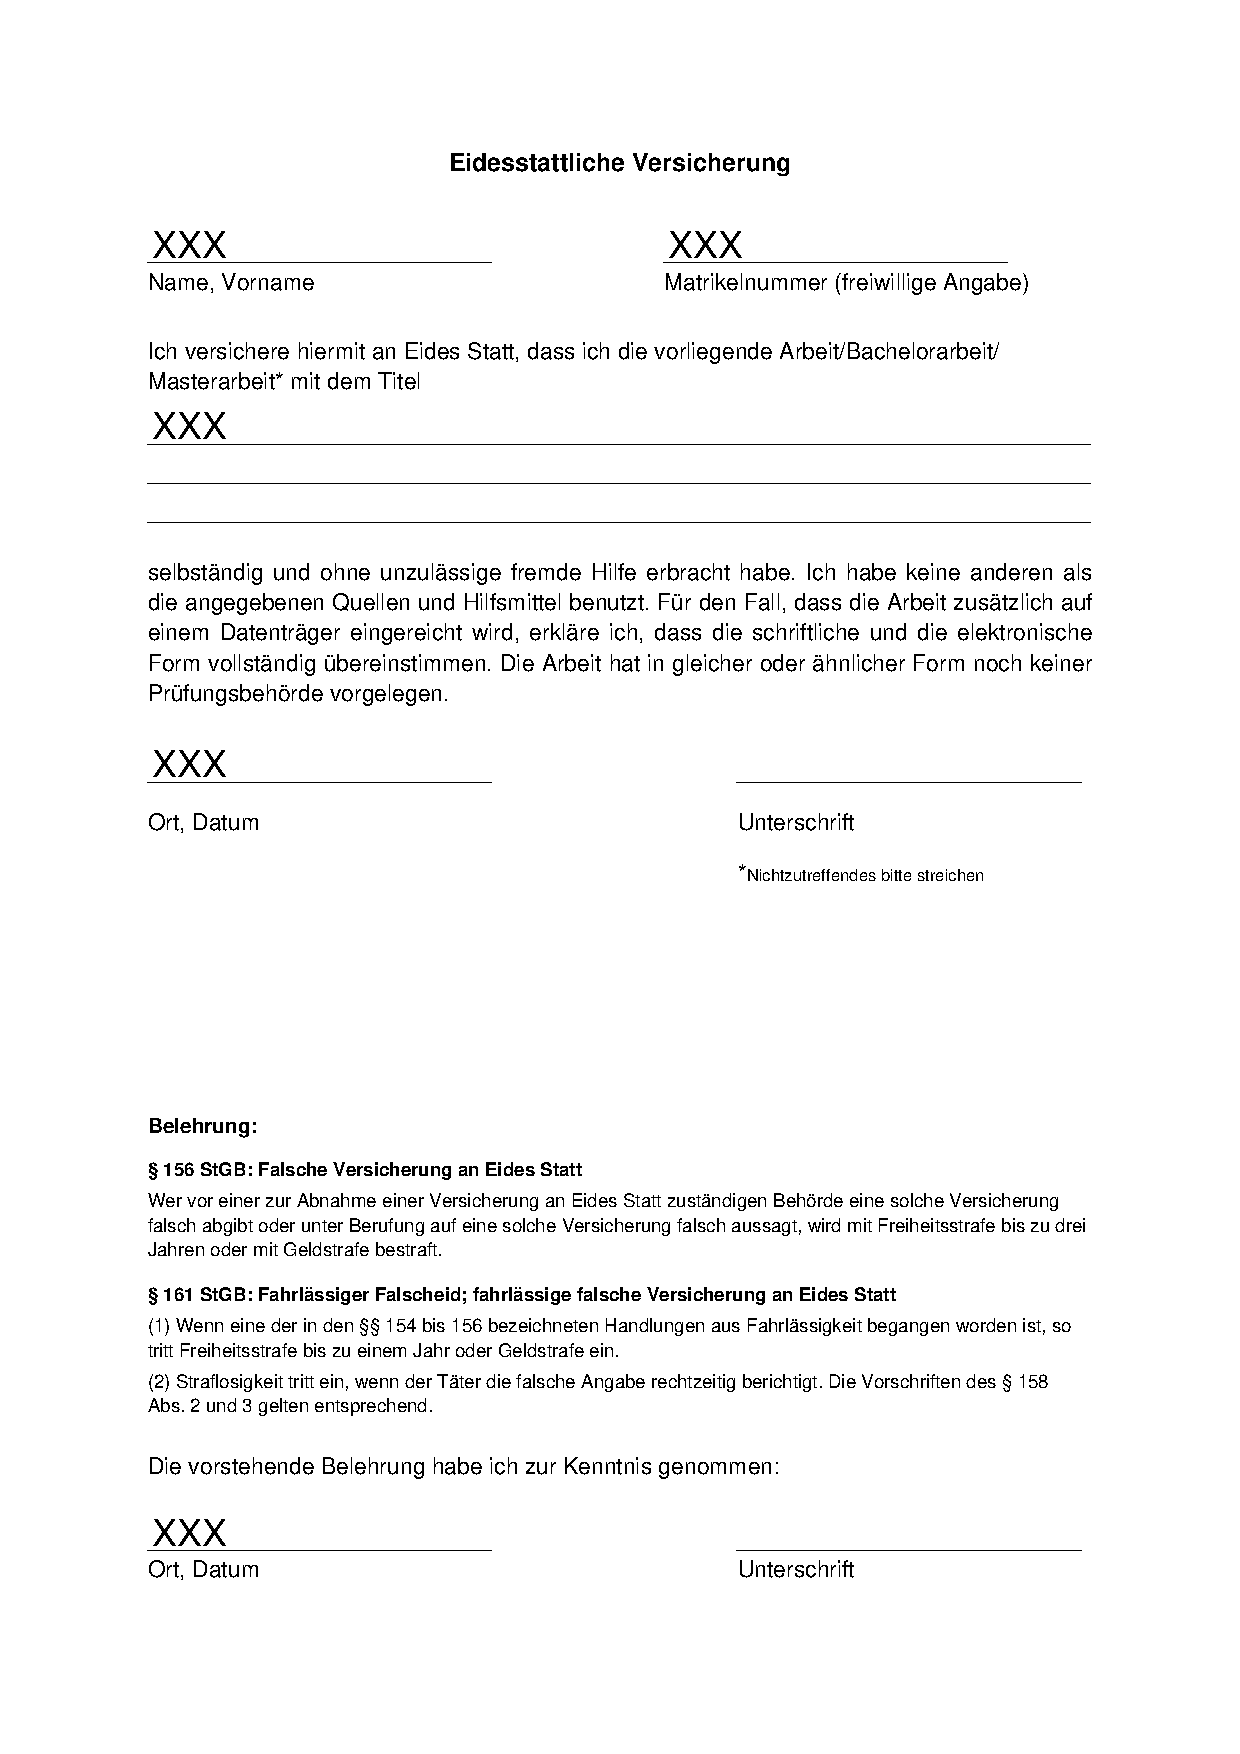
\includegraphics[width=0.95\linewidth, trim={2.5cm 3cm 2.5cm 4cm}, clip]{Formular_Eidesstattliche_Versicherung}};
\node [anchor=south west, inner sep=0] at (0cm, 18.4cm) {\Large \Surname, \Firstname};
\node [anchor=south west, inner sep=0] at (7.2cm, 18.4cm) {\Large \MatrikelNummer};
\node [anchor=south west, inner sep=0] at (0cm, 15.9cm) {\large \makeatletter \@title \makeatother};
\node [anchor=south west, inner sep=0] at (0cm, 11.2cm) {\large \Aachen, \publicationDate};
\node [anchor=south west, inner sep=0] at (0cm, 0.5cm) {\large \Aachen, \publicationDate};
\draw [line cap=round, line width=0.5mm] (8.8cm, 17.11cm) -- (9.65cm, 17.11cm); % cross out "Arbeit"
\draw [line cap=round, line width=0.5mm] (9.75cm, 17.11cm) -- (11.70cm, 17.11cm); % cross out "Arbeit"
%\draw [line cap=round, line width=0.5mm] (0cm, 16.7cm) -- (1.8cm, 16.7cm); % cross out "Masterarbeit"
\end{tikzpicture}
% \end{center}


% \includegraphics[width=0.95\linewidth, trim={2.5cm 2.9cm 2.5cm 3.9cm}, clip]{Formular_Eidesstattliche_Versicherung_neu}

} 
\graphicspath{ {./figures/} }
\selectlanguage{british}
\chapter{Abstract}
In recent years, cross-lingual representation of words enable us to explore the structures of different languages, based on that similarity we can realize bilingual dictionary induction and information retrieval, it also enable the knowledge transfer bwtween languages especially between resource-rich and resource-lean languages.\\
In this thesis we first make a survey of the cross-lingual word embedding training methods and its application in unsupervised machine translation. Then we proposed a novel training method of cross-lingual word embedding, which is data-driven and supported with language model, we can better utilize the context information for training. we further exploit the cross-lingual similarity in word-by-word based unsupervised machine translation combined with context-aware beam search and denoising autoencoder. \\
The performance of the cross-lingual embedding is measuared on an open dictionary from Facebook, we find the performance is comparable with the state-of-the-art supervised and unsupervised methods. Based on that, our simple yet efficient unsupervised machine translation system can produce meaningful machine translation the BLEU scores even get beyond some unsupervised system with costly iterative training. \\
We also make some ablation studies, analyze the effects of various factors in the cross-lingual word embedding training and various artificial noise. We think our work can provide better understanding of the training and the applications of word embedding in MT.

%\input{acknowledgements}

\pdfbookmark[0]{Contents}{toc} % ziffer fuer ebene
\glsunsetall
\tableofcontents

\mainmatter          % Hauptteil (arabische Seitenzahlen)

\glsresetall

\chapter{Introduction}
Building a good machine translation (MT) system requires an enormous collection of parallel data. Neural machine translation (NMT) systems has emerged as the
most promising machine translation approach in recent years, showing superior performance on public benchmarks and rapid adoption in deployments. However MT systems often fail when the training data is not enough. However, parallel corpora are expensive because they require huge human labor, time and expertise of corresponding languages.
\indent Several approaches has been proposed to alleviate this issue, for instance, triangulation or semi-supervised learning techniques; these systems however still need a strong cross-lingual signal. Unsupervised MT uses only monolingual data of the source and target languages to train the model and in fact, monolingual corpora are readily available.\\
Recently, cross-lingual word embedding draws more and more attention since it helps to explore the multilingual semantic information in a shared space. For instance, it enables computation of cross-lingual word similarities, which  can be directly applied to bilingual dictionary induction or cross-lingual information retrieval. Several methods are proposed to learn the cross-lingual cross-lingual word embedding without any parallel data. This correspondingly inspires work on unsupervised MT.\\
In this thesis, I propose a novel corpus-based unsupervised training method, the experiments the method can achieve competitive results  in comparison with the start-of-the-art methods. I further explore the 
application of the cross-lingual word embeddings in the MT task.
I develop a fully unsupervised MT system starting from the simple word-by-word translation principle. Language model (LM) is integrated to improve the translation. In order to boost the translation efficiency, I design a context-aware beam search to find the best translation candidate. To handle to reordering, I implement a denoising network with artificial noises, which are to mimic the true noises in the word-by-word translation, The results demonstrate that such simple but efficient translation system performs better even than most unsupervised neural MT system with costly iterative training.


\section{Related Work}

\subsection{Word Embedding}
\indent Traditional language processing systems treat words as discrete atomic symbols, which assign for each word a specific ID number. Such encodings are arbitrary; it does not provide any information about the relations that may exist between individual symbols. In comparison, distributed representations of words in a high dimensional continuous space help learning algorithm to achieve better performance in natural language processing. According to the distributional hypothesis, similar words tend to occur with similar neighbors, and have similar word representations. \\
\cite{mikolov2013efficient} propose two models for learning word embeddings with neural networks, namely skip-gram and continuous bag of words (CBOW) models. Neural architectures makes the training extremely efficient. In further work, \cite{mikolov2013distributed} discuss about learning the embedding for phrases. \cite{pennington2014glove} propose a regression model which combines the global matrix factorization and local context window methods, making the training process more interpretable. \cite{DBLP:journals/corr/BojanowskiGJM16} represent each word as a bag of character $n$-grams, and assign for each character $n$-gram a distinct embedding. In this way, they can exploit subword information. \\
\cite{mikolov2013exploiting} notice that continuous embedding spaces exhibit similar structures across languages, even for distant language pairs, for example, English-Vietnamese.  With separately learned monolingual embeddings they learn a linear mapping from source embedding space to target embedding space. To do this, they employ a parallel vocabulary of five thousand words as anchor points and evaluate their approach on a word translation task. \cite{xing2015normalized} show that results can be improved by enforcing an orthogonal constraint on the linear mapping. \\
Recently, \cite{artetxe2017learning} raise an iterative method that aligns the word embedding spaces gradually. In their work, the vocabulary size for learning can be reduced to 25 word pairs and even only with Arabic numerals. The performance is comparable to the learning with large vocabulary dictionary \cite{cao2016distribution} propose a distribution-based model, which is a modified CBOW model minimizing the distribution dissimilarity between source and target embeddings; here, distribution information refers the mean and variance. 
\cite{zhang2017adversarial} put forward  a method using adversarial training without any parallel data. The discriminator tries to distinguish if the embedding is from the source side, the generator aims to learn the mapping from source embedding space to the target one. These methods are fully unsupervised but the performances are far from the supervised training. \cite{DBLP:journals/corr/abs-1710-04087} simplify the adversarial training structure with different loss functions for the generator and discriminator, regularize the linear mapping to be orthogonal, the results get improved significantly. They also propose to use cross-domain similarity local scaling (CSLS) to handle hubness.

\subsection{Unsupervised MT}

As mentioned previously, the lack of parallel corpora motivates people to use monolingual data to improve the MT system. Some researchers use triangulation techniques (\cite{cohn2007machine}) and semi-supervised approaches (\cite{DBLP:journals/corr/ChengXHHWSL16}) to alleviate this issue. But these methods still require parallel corpora.\\
As to fully unsupervised MT, which only takes advantage of monolingual data, \cite{ravi2011deciphering} first consider it as a deciphering problem, where the source language is considered as ciphertext. They also propose iterative expectation-maximization (EM) method and Bayesian decipherment to train this unsupervised model. To solve the bottleneck of such model; mainly the huge memory required to store the candidates search space, \cite{nuhn2012deciphering} limit search candidates according to the word similarity. \cite{nuhn2014decipherment} limit the search space by using and preselection beam search. For the same reason, \cite{kim2017unsupervised} enforce the sparsity with a simple thresholding for the lexicon, also initializing the training with word classes to efficiently boosts the performance. 
Although initially not based on distributional semantics, recent studies show that the use of word embeddings can bring significant improvement in statistical decipherment (\cite{duong2016learning}).\\
For neural MT, \cite{he2016dual} show a bidirectional, iterative way of effectively using monolingual data. More concretely, they train two agents to translate in opposite directions (e.g. French ${\leftrightarrow}$ English) and make them teach each other through a reinforcement learning process. While promising, this approach still requires a small parallel corpora for a warm start.  
\cite{artetxe2017unsupervised} and \cite{lample2017unsupervised} propose two bi-directional unsupervised MT models which totally rely on monolingual corpora in each language only. Both models need to use cross-lingual word embedding to initialize the MT system and train the sequence-to-sequence system with denoising autoencoder. By introducing back-translation techniques, they turn the unsupervised training into a supervised one. The most important principle for these two work is the shared representations. Sentences from different languages are encoded into a shared spaces.
\section{Outline}
The remainder of this thesis is structured as follows. In Section 1.3 we introduce the notations for this thesis. 
Chapter 2 introduces the development of MT systems from statistical models to  neural models. Some basic techniques and principles for unsupervised MT are also explained.  Chapter 3 gives a survey of training and applications details of cross-lingual word embedding. Chapter 4 discusses the unsupervised learning of cross-lingual word embedding and our efforts on data-driven training. We describe our unsupervised MT system in Chapter 5, which contains mainly context-aware search with the help of language model and denoising autoencoder method aimed at reordering. We demonstrate experimental results of cross-lingual word embedding model and unsupervised machine system in Chapter 6, comparing the performance with the state-of-the-art model. In Chapter 7, we summarize our work and draw conclusions.


\section{Notation}
In this thesis, we use the following notations:
\begin{itemize}
	\item Source sentence:  ${f_1^J:= f_1 \cdots  f_j \cdots f_J}$ 
	\item Target sentence:  ${e_1^I:= e_1 \cdots, e_i \cdots e_I}$
	\item Parallel sentences: $(e_1^I, f_1^J)$
	\item Probabilities of denoising autoencoders: $p_{f\rightarrow f}$, $p_{e\rightarrow e}$
	\item Translation models for both directions: $\Theta_{f\rightarrow e}$, $\Theta_{e \rightarrow f}$
	\item Probabilities of translation models for both directions: $p_{f\rightarrow e}$, $p_{e\rightarrow f}$
	\item Loss for denoising autoencoder: $\mathcal{L}^{\text{auto}}$
	\item Loss for back-translation: $\mathcal{L}^{\text{back}}$
	\item Single character for each language: $f,e$ 
	\item Source and target word embedding: $\bm{f}$, $\bm{e}$
	\item Seed bilingual dictionary: $dico$ 
	\item Corresponding embedding pair: $(\bm{f}, \bm{e})$
	\item Alignment: a
	\item Source and target embedding matrices: $\bm{F}$, $\bm{E}$
	\item Source and target Corpora: $\mathcal{F}, \mathcal{E}$
	\item Mapping default from source to target embedding space: $W$
	\item Mapping with specific direction: $W_{f\rightarrow e}$, $W_{e\rightarrow f}$
	\item Internal states of decoder: $\bm{s}$ and $\bm{s}_i$  
	\item Internal states of encoder: $\bm{h}$ and $\bm{h}_i$ 
	\item Context vectors in attention mechanism: $\bm{c}$ and $\bm{c}_i$ 
	\item Learnable matrices related with context vector, hidden state and alignment: $W_c, W_s, W_a$ 
	\item Cross-lingual regularization term $\Omega(\cdot)$
	\item Loss function for source and target embedding: $\mathcal{L}^f$, $\mathcal{L}^e$
	\item Temperature in inverted softmax: $\beta$ 
	\item General scaling parameter: $\lambda$
	\item Scaling parameters for lexicon and languagel model respectively: $\lambda_{lex}$, $\lambda_{LM}$
	\item Expectation: $\mathbb{E}$
	\item Dimension of embedding: $d$
	\item Neighbors of source and target cross-lingual embeddings: $\mathcal{N}_{e}(\bm{f})$, $\mathcal{N}_{f}(\bm{e})$, 
	\item Frobenius norm: ${\lVert \cdot \rVert}_{\text{F}}$
	\item  Manifold of orthogonal matrices: $ O_d(\mathbb{R})$
	\item Language model for source and target size: $\textbf{LM}_f$, $\textbf{LM}_e$
	\item Similarity matrices for source and target respectively: $M_F$,$M_E$
	\item Vocabulary size for most frequent words ${\lvert \tilde{V} \rvert}$
	\item Permutation distance: $d_{per}$
	\item Probability of deletion noise: $p_{del}$, of insertion noise: $p_{ins}$
	\item Vocabulary size for insertion noise  $V_{ins}$  
	\item Model score not exact the probability, especially in weighted model: $Q(\cdot)$
	\item Feature functions: $q(\cdot)$
	\item Discounting coefficient in phrase detection: $\delta$
\end{itemize}











%\cite{mikolov2013distributed}
%\cite{artetxe2017unsupervised}


\glsresetall
\chapter{Machine Translation}
This chapter describes the classical or start-of-the-art machine translation models from statistical machine translation model to neural machine model. The relative research works on unsupervised machine translation will also be included.


\section{Statistical Machine Translation}
%%%
%The initial models for machine translation are based on words as units (Word-based machine translation), that can be translated, inserted, dropped and reordered.
%Fertility is the notion that input words produce a specific number of output words in the output language.
%
%Define the phrase-based statistical machine translation model mathematically.  First apply the Bayes rule to invert the translation direction and integrate a language model $p_{LM}$ so the best English translation for the input sentence ${f} $ is defined as 
%
%The advantages of the phrase-based machine translation is :
%\begin{enumerate}
%	\item many-to-many translation can handle non-compositional phrase	
%	\item better utilization of local context in translation
%	\item the more data, the longer phrases can be learned 
%\end{enumerate}
Statistical machine translation has achieved success until the beginning of this century. The initial statistical models for machine translation are based on words as atomic units that may be translated, inserted, dropped and reordered. In statistical machine translation, we use both a translation model and a language model which ensures fluent output. Later the statistical machine translation prefers to use translation of phrases as atomic units. These phrases are any contiguous sequences of words, not necessarily linguistic entities. In this approach, the input sentence is broken up into a sequence of phrases, these phrases are mapped one-to-one to output phrases, which may be reordered.

\subsection{Word-Based Model}
\noindent \textbf{Noisy-channel model:}
Noisy channel model based on the notion of a noisy channel from Shannon's information theory has been applied to many language processing problems. Assume the source sentence is a distorted message omitted from the target sentence, we have a model on  how the message is distorted (translation model $Pr(f_1^J|e_1^I)$) and also a model on which original messages are probable (language model ${Pr(e_1^I)}$), our task is to find the best translation ${e_1^I}$ for an input foreign sentence.
\begin{align*}
\argmax{e_1^I} \{Pr(e_1^I | f_1^J)\} & = \argmax{e_1^I} {\frac{Pr(f_1^J | e_1^I)Pr(e_1^I)}{Pr(f_1^J)}} \\
& = \argmax{e_1^I} { \{ Pr(f_1^J | e_1^I) \cdot  Pr(e_1^I)\} }
\end{align*} 


The basic model for word-based model is noisy-channel model. The task of word alignment is an artifact of word-based machine translation. Alignment models target at the reordering problem for word-based translation.\\

\subsubsection{IBM Models}
Based on the noisy-channel model, IBM word-based translation make the model more complicated by adding submodels. Starting from lexical translation, absolute alignment model, fertility etc. are added step by step.\\

 \textbf{Alignment model} introduce an explicit model for reordering words in a sentence. More often than not, words that follow each other in one language have translations that follow each other in one language have translations that follow each other in the output language. In detail, the position $j$ in the source sentence is aligned with the position $i$ in the target sentence when translating, denoted as  ${i=a_j}$. Alignment model is a global reordering model.For whole sentence, we denote the alignment as 
\[a_1^J:= a_1\cdots a_J\]

\textbf{Fertility model} the specific number of output words in the output language. Generally one word in one language just translate into one single word in the other language. But some words produce multiple words or get dropped. we denote the fertility model as $\phi(e)$, so the length of translation sentence  
\[ J = \sum_{i=0}^{I} \phi(e_i) \]

The word-based translation process can be described as the following figure, we use IBM-3 model for example:  
IBM-3 model contains four steps: 
\begin{itemize}
	\item Fertility step
	\item NULL insertion
	\item Lexical translation step
	\item Distortion step for reordering
\end{itemize}
\begin{figure}[t]
	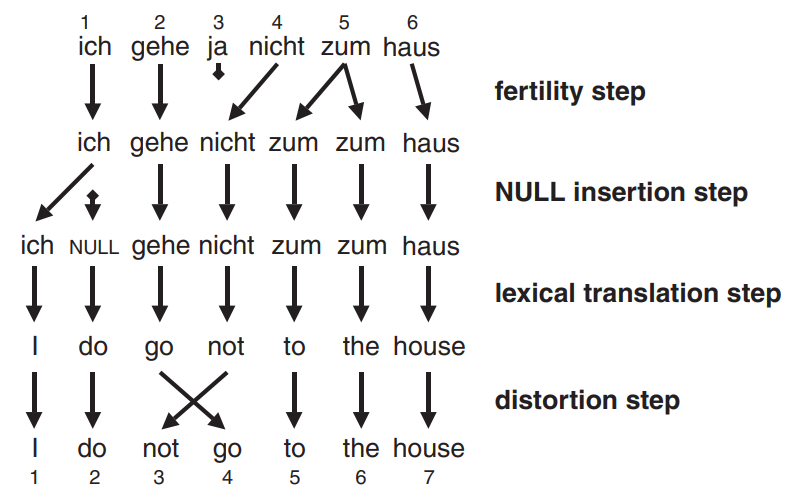
\includegraphics[width=12cm]{wordsmt}
	\caption{ Illustration of IBM-3 model (\cite{koehn2009statistical})}
	\centering
\end{figure}




\subsubsection{Weighted Model}
To overcome shortcomings in modeling, introduce scaling exponents ${\lambda_{m}}$ as in speech recognition. For example
\[ Q(f_1^J, e_1^I; a_1^J) = P(J|I)^{\lambda_1} \cdot \prod_{i} P(e_i|e_h)^{\lambda_2} \cdot \prod_{j} [p(a_j|a_{j-1}, I, J)^{\lambda_{3}} \cdot p(f_j|e_{a_j})^{\lambda_4}]  \]
where the four probabilities corresponds to length model, language model, alignment model and lexical model separately. $e_h$ denotes the history words in $N$-gram model



\subsection{Phrase-Based Model}
Actually when translating, words may not be the best candidates for the smallest units for translation, sometimes one word in a foreign languages should be translated into two English words, or vice versa. Word-based models often break down in these cases.\\
Phrase-based models typically do not strictly follow the noisy-channel approach proposed for word-based models, but use a log-linear framework This model allow s straightforward integration if additional features.\\

\textbf{Log-linear Model Combination}:
Consider arbitrary models ("feature functions"):
\[ q_m(f_1^J, e_1^I; a_1^J) > 0  \quad m = 1, \cdots, M\]

\begin{align*}
	Q(e_1^I, f_1^J; a_1^J) & = \prod_{m=1}^{M} q_m(f_1^J, e_1^I; a_1^J)^{\lambda_m} \\
	& = \exp(\sum_{m=1}^{M} \lambda_m \log q_m(f_1^J, e_1^I; a_1^J))
\end{align*}
In this frame work, we view each data point as a vector of features and the model as a set of corresponding feature functions, these functions are trained separately and combined assuming that they are independent of each other.\\ 

Components for log-linear model can be such as language model, phrase translation model, reordering model are used as feature functions with appropriate weights.
\begin{itemize}
	\item Phrase translation model can be learned from a word-aligned parallel corpus, alternatively we also can use expectation maximization algorithm to directly find phrase alignment for sentence pairs.
	\item Reordering model for phrase case is typically modeled by a distance based reordering cost that discourage reordering in general. Lexicalized reordering model can be introduced for specific phrase pair.
\end{itemize}

The model can be further extended by components like: bidirectional translation probabilities, lexical weighting, word penalty and phrase penalty. 

\subsection{Decipherment}
\cite{ravi2011deciphering} frame the MT problem as a decipherment task, treating the foreign text as a cipher. They also propose iterative expectation-maximization method  (EM) and Bayesian decipherment to train this unsupervised model. Many concepts in deciperment are the same as the SMT.\\

IBM model tries to maximize the probability with hidden alignment model
\[ \argmax{\theta} \prod_{\bm{e}, \bm{f}} {P_{\theta}(\bm{f}|\bm{e})} = \argmax{\theta} \prod_{\bm{e}, \bm{f}} \sum_{a} P_{\theta}(\bm{f}, a| \bm{e})  \]
While for unsupervised case, we train 
\[ \argmax{\theta} \prod_{\bm{f}}P_{\theta}(\bm{f})= \argmax{\theta} \prod_{\bm{f}} \sum_{\bm{e}} P(\bm{e}) \cdot P_{\theta}(\bm{f}|\bm{e})\]

for hidden alignments: \[ \argmax{\theta} \prod_{\bm{f}} \sum_{\bm{e}} P(\bm{e}) \cdot \sum_{a} P_{\theta}(\bm{e},a|\bm{e}) \]

Since the model is very complicated, more assumptions are added to the model. The model accounts for word substitutions, insertions, deletions and local reordering during the translation process but does not incorporate fertilities or global re-ordering.\\

The generative process:
\begin{enumerate}
	\item Generate an English sentence $\bm{e}$ with probability $P(\bm{e})$.
	\item Insert a NULL word at any position in the English sentence with uniform probability.
	\item For each English word token $e_i$ (including NULLs), choose a foreign word translation $f_i$, with probability $P_{\theta}(f_i| e_i)$, the foreign word may be NULL.
	\item Swap any pair of adjacent foreign words $f_{i-1}, f_i$, with probability ${P_{\theta}(swap)}$. 
	\item Output the foreign string $f_1^M$, skipping over NULLs.
\end{enumerate}

However, this method is limited to rather short sentences and simplistic settings.
\section{Neural Machine Translation}
Neural machine translation (NMT) has recently become the dominant method for machine translation task. In comparison to the traditional statistical machine translation (SMT), NMT systems are trained end-to-end, taking advantages of the continuous representation of the hidden states that greatly alleviate the sparsity problem and make better use of more contextual information. Besides this, traditional phrase-based machine translation, which consists of several models that are tuned separately, neural machine translation tries to build a more general neural network model which can directly output translations given input, it contains only one single model, and only one single training criterion. \\
\cite{sutskever2014sequence} first use a multi-layer Long Short-Term Memory (LSTM) to to train the machine translation system, attention mechanism has lately been used to improve neural machine translation by selectively focusing on parts of the source sentence during translation. The inherently sequential nature precludes parallelization within training examples. Convolutinoal sequence to sequence (ConvSeq2seq) and Transformer architectures are brought forward  for significantly more parallelization during training to better exploit the GPU hardware and these models can reach a new state of the art in
translation quality.


\subsection{Encoder-Decoder Framework}
\begin{figure}[t]
	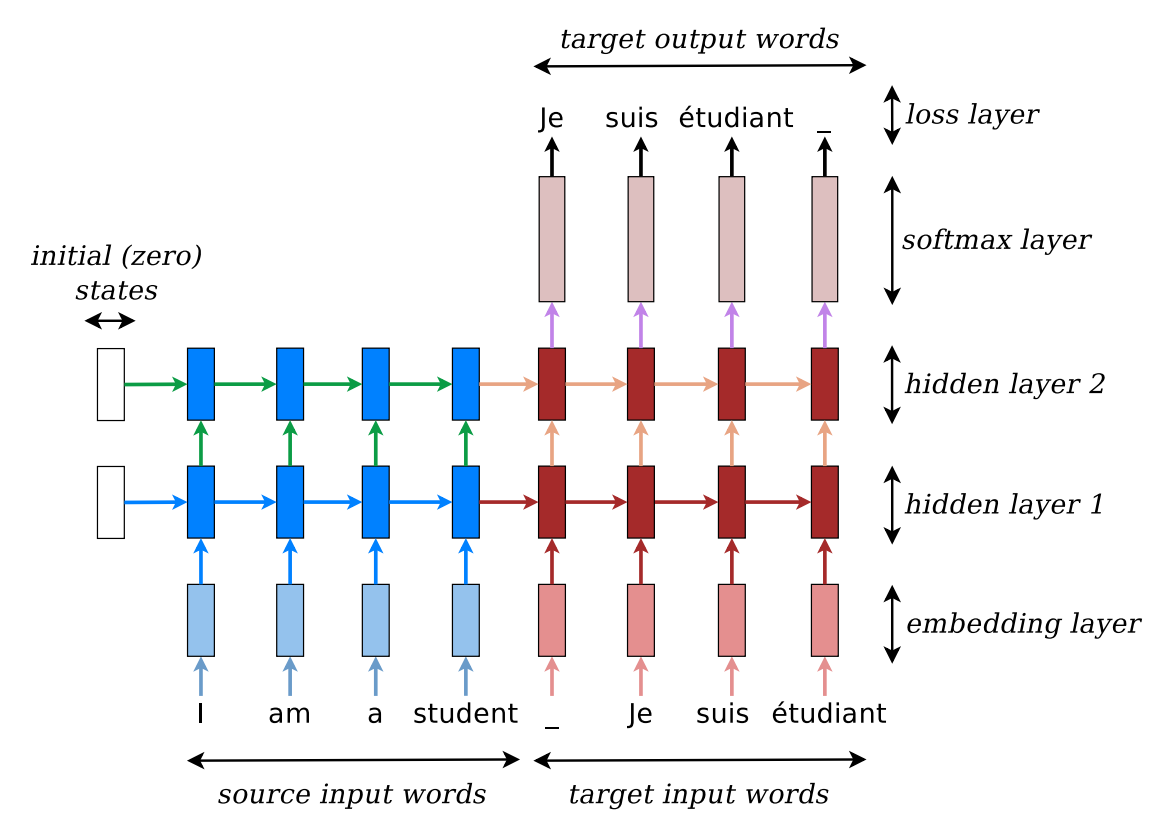
\includegraphics[width=12cm]{nmt}
	\caption{ Neural machine translation – example of a deep recurrent architecture (\cite{luong2015effective})}
	\centering
\end{figure}

The most common network structure is the encoder-decoder framework, in which two recurrent neural networks work together to transform one sequence to another. An encoder condenses an input sequence into a vector $\bm{c}$, and a decoder unfolds that vector into a new sequence. The model can be expressed as:
\[ p(e_1^I | f_1^J) = \prod_{i} p(e_i|e_0^{i-1}, f_1^J) = \prod_{i} {p(e_i|e_0^{i-1},  {\bm{c}})} \] 

%The final hidden and cell state from the encoder is used to initialize the state of the decoder. This means every time that the encoder model encodes an input sequence, the final internal states of the encoder model are used as the starting point for outputting the first character in the output sequence.
 The RNN decoder predicts the next word on the basis of the internal states and the previous word. In more detail, one can parameterize the probability of decoding each word $e_i$ as:
 \[ p(e_i|e_0^{i-1},  {\bm{c}}) = \text{softmax}(g(\bm{s_i}))\]
 with $g$ being the transformation function that outputs a vocabulary-size vector. Here $\bm{s}_i$ is the RNN hidden state, updated as:
\[ \bm{s}_i = f(\bm{s}_{i-1}, \bm{c})\]

It is common in neural machine translation systems to use a beam-search to sample the probabilities for the words in the sequence output by the model. The wider the beam width, the more exhaustive the search, and, it is believed, the better the results.\\









%
%\[ p(e_t|e_{t-1} h_{t-1}, f_1^J) =  p(e_t| e_{t-1}, h_{t-1}, c_t)\]
%
%\[ \bm{\tilde{h_{t}}} = tanh(\bm{W_{c}[c_t; h_t]}) \]
%\[p(y_t| y_{<t}, x) = \text{softmax}(\bm{W_s \tilde{h_t}})\]

\textbf{Drawbacks}:
\begin{enumerate}
	\item The model compresses all information from the input sentence into a hidden vector ${1}$, while ignores the length of input sentence, when the length of input sentence get very long, even longer than the training sentences, it becomes harder to extract specific information for predicting the target word, the performance will get worse.
	\item It's not suitable to assign the same weight to all input words, one target word corresponds usually to one or several words in the input sentence. Treating all words equally does not distinguish the source information and influence the performance badly.

\end{enumerate}

\subsection{Attention Mechanism}
Alignment is the problem in machine translation that identifies which parts of the input sequence are relevant to each word in the output, whereas translation is the process of using the relevant information to select the appropriate output.
\cite{bahdanau2014neural} introduce an extension to the encoder-decoder model which learns to alignment and translate jointly. Each time the model predicts the next target word, it softly searches for a set of positions in a source sentence where the most relevant information is concentrated. The model then predicts a target word based on the context vectors associated with these source positions and all the previous generated target words.\\
Described in formula, attention mechanism derives a context vector ${\bm{c}_i}$ that capture the input information to help to predict the target word at the position ${i}$. Given the target hidden state ${\bm{s}_i}$ and the source-side context vector $\bm{c}_i$, we can compute the hidden state ${\tilde{\bm{s}}_i}$ by combining the current hidden state $\bm{s}_i$ and the context vector $\bm{c_i}$:
\[ \tilde{\bm{s}}_i = tanh(W_c[\bm{c}_i; \bm{s}_i])\]

Then the target word is correspondingly predicted by softmax function:
\[  p(e_i|e_0^{i-1}, f_1^J) = softmax(W_s \tilde{\bm{s}}_i)\] 
%\begin{figure}
%	\begin{minipage}[h]{0.5\textwidth}
%		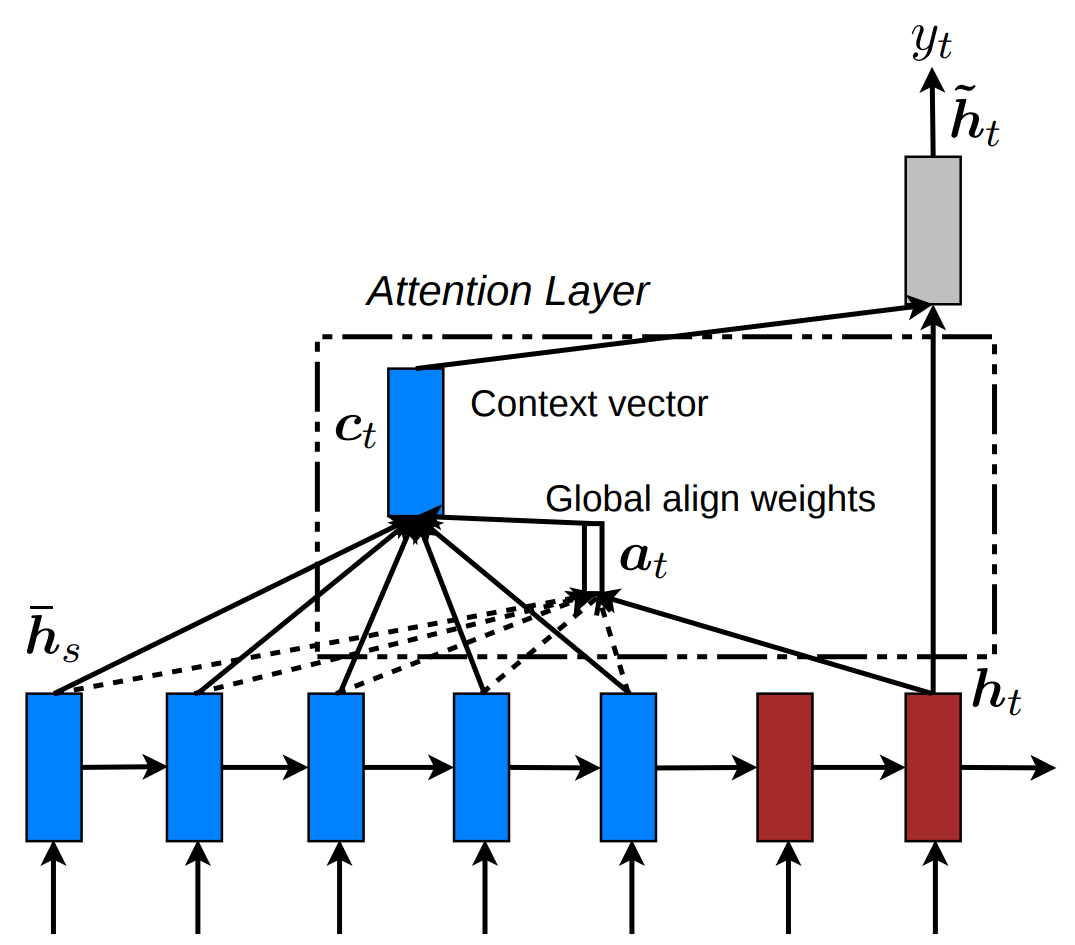
\includegraphics[width=\textwidth]{attentiong.png}
%		\caption{Picture 1}
%		\label{fig:1}
%	\end{minipage}
%	
%	\begin{minipage}[h]{0.5\textwidth}
%		includegraphics[width=textwidth]{attentionl.png}
%		\caption{Picture 2}
%		\label{fig:2}
%	\end{minipage}
%\end{figure}
\begin{figure}
	\centering
	\begin{minipage}{.5\textwidth}
		\centering
		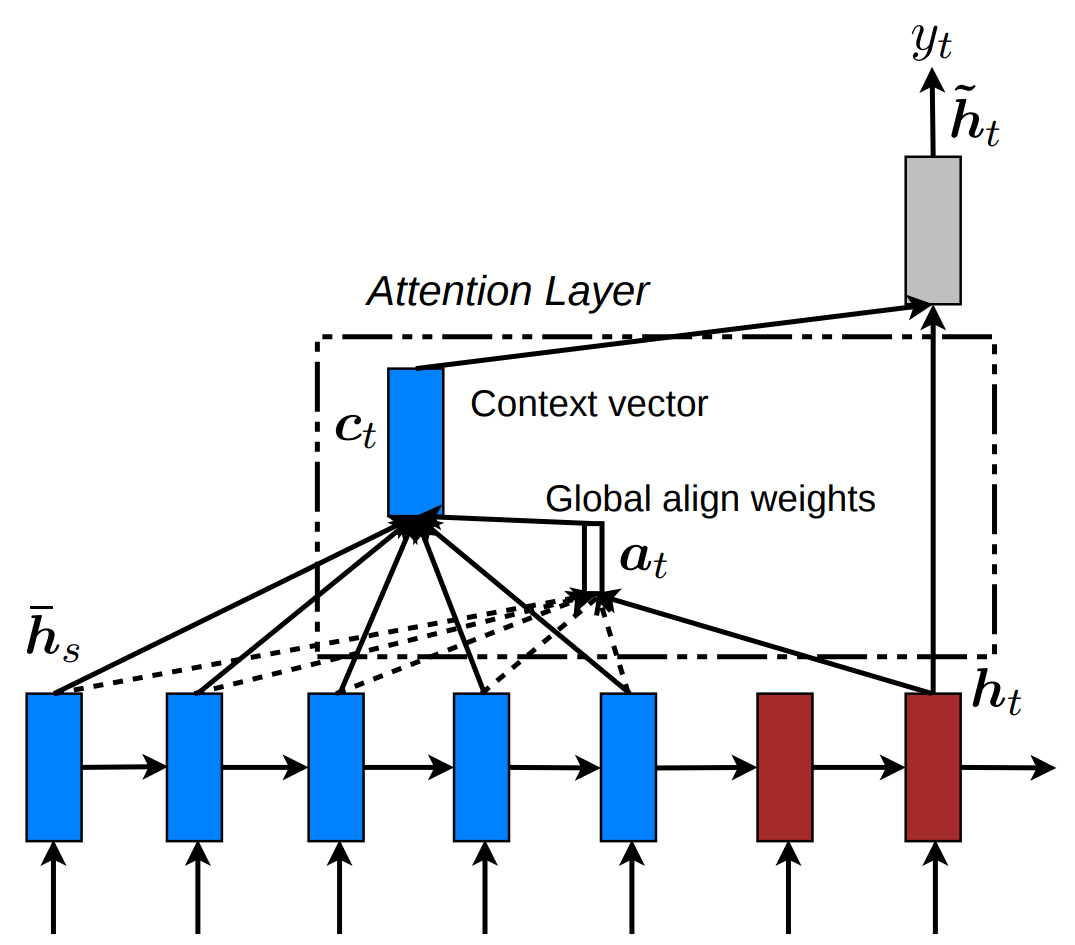
\includegraphics[width=1\linewidth]{attentiong}
		\captionof{figure}{Global attention}
		\label{fig:test1}
	\end{minipage}%
	\begin{minipage}{.5\textwidth}
		\centering
		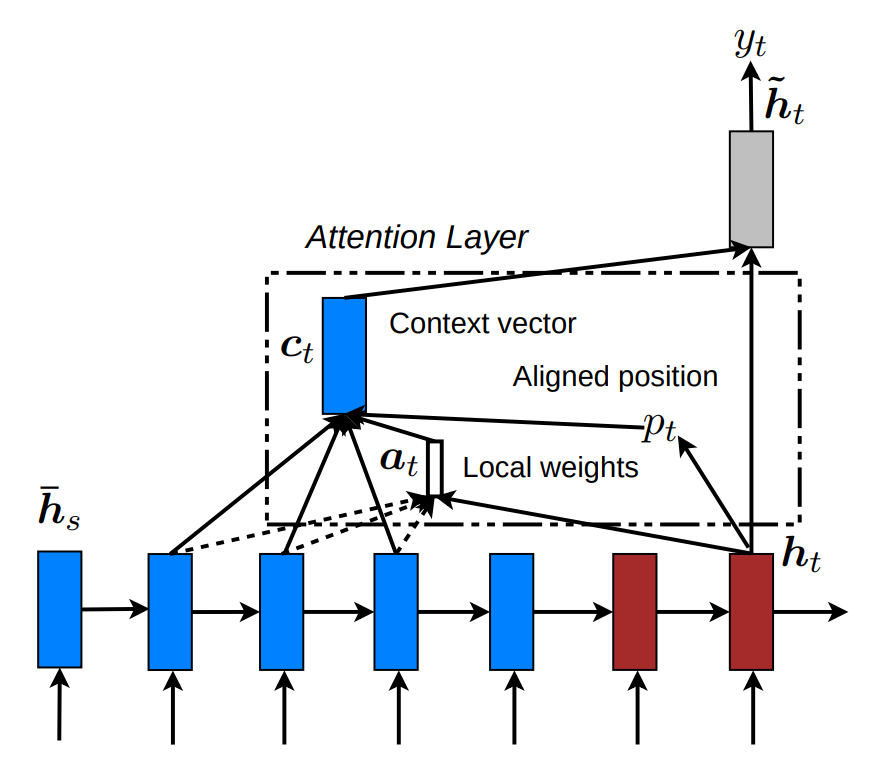
\includegraphics[width=1\linewidth]{attentionl}
		\captionof{figure}{Local attention}
		\label{fig:test2}
	\end{minipage}
\end{figure}
%\begin{figure}[t]
%	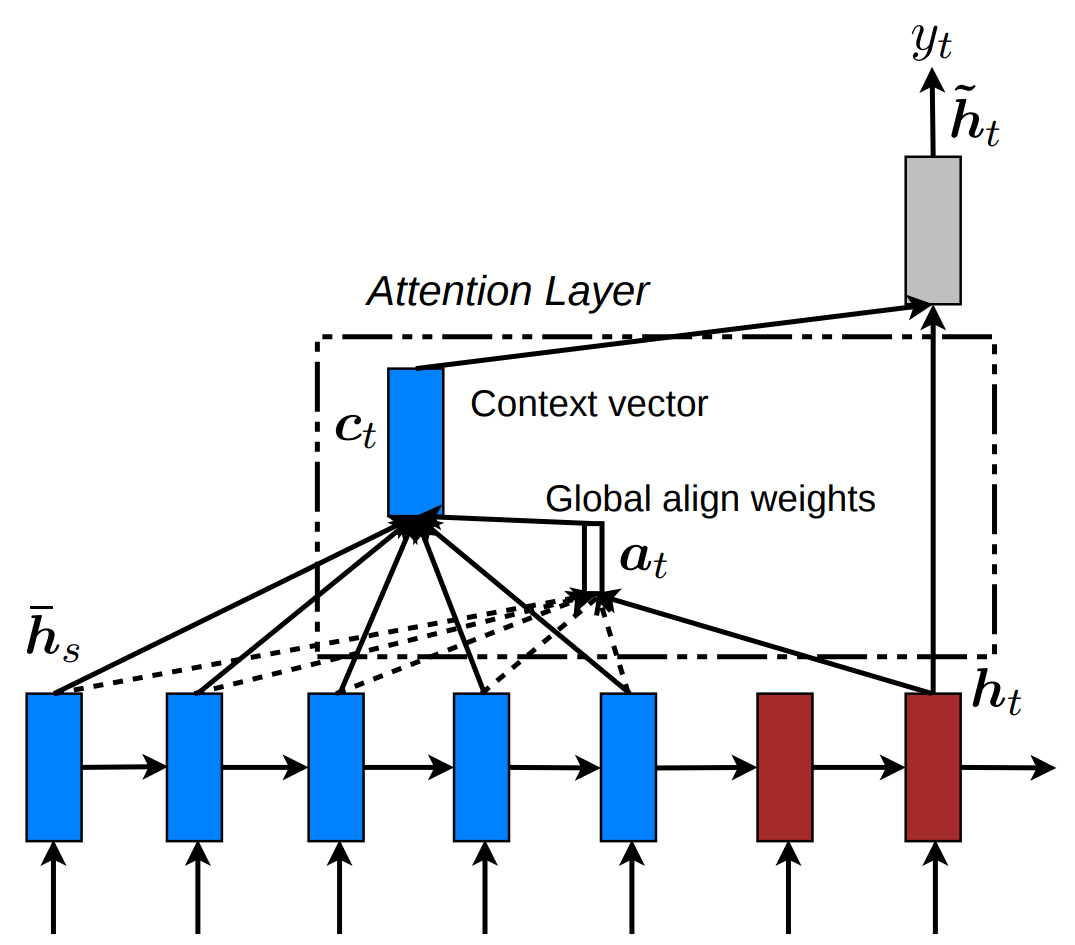
\includegraphics[width=6cm]{attentiong}
%	\caption{Global attention model (\cite{luong2015effective})}
%	\centering
%\end{figure}
%
%\begin{figure}[t]
%	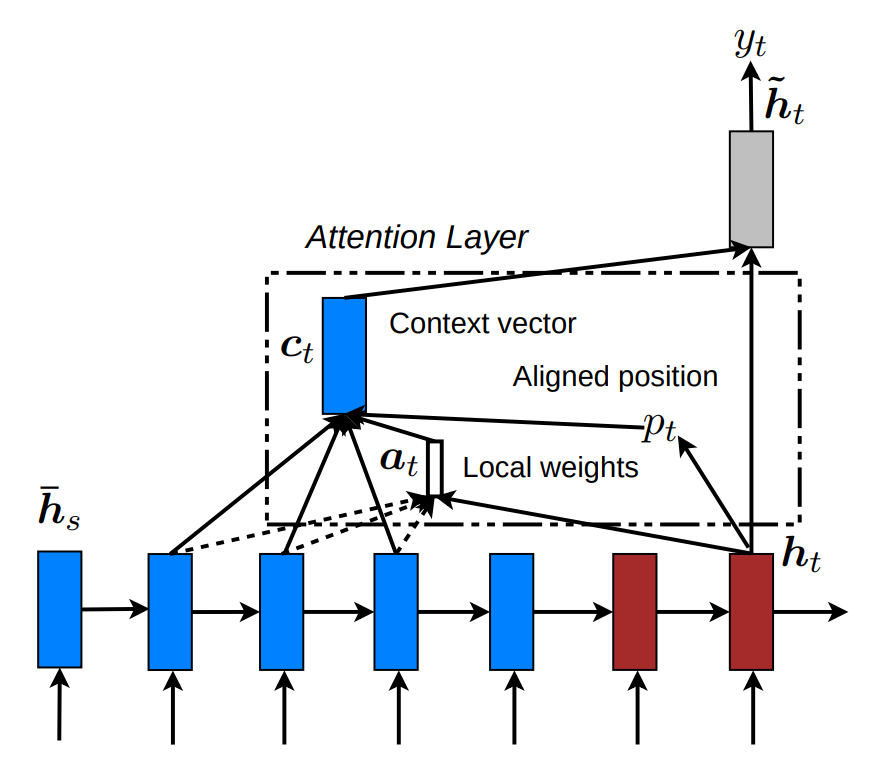
\includegraphics[width=6cm]{attentionl}
%	\caption{Local attention model (\cite{luong2015effective})}
%	\centering
%\end{figure}


\textbf{Global attention \& Local attention } \\
\textbf{Global attention} attends all the input words, weighted average of source hidden states (word representations):
\[ \bm{c}_i = \sum_{j} \bm{\alpha}(j|i)\cdot  \bm{h}_j \]
where $\bm{\alpha}(j|i)$ is the normalized attention weight that output at position $i$ is aligned with input position $j$, and it can be calculated as the following softmax-like function:
\begin{align}
\bm{\alpha}(j|i) = & \ \text{align}(\bm{s}_i, {\bm{h}}_j) \\
= & \ \frac{\text{exp\ }(\text{score}(\bm{s}_i, {\bm{h}}_j))}{\sum_{\bm{j}^{\prime}} \text{exp\ }(\text{score}(\bm{s}_i, {\bm{h}}_j^{\prime}))}
\end{align}
Since score function is referred as a content based function, different forms can be considered:
\begin{equation}
\text{score}(\bm{s_i}, {\bm{h}}_j)=\left\{
\begin{array}{lcl}
{\bm{s_i}}^T {\bm{h}}_j & & dot\\
{\bm{s_i}}^T W_a {\bm{h}}_j & & general\\
{\bm{v_i}}^T tanh(W_a[\bm{s_i}; {\bm{h}}_j]) & & concat
\end{array} \right.
\end{equation}



For global attention, for each target word we need to attend the whole input sentence, it is very expensive and impractical to translate longer sentences. \cite{luong2015effective}) proposed the local attention, the local attention is actually the  trade-off between soft and hard attention. \\
\textbf{Local attention} first predicts an aligned position ${a(i)}$ for each target word at position $i$. Then the context vector ${\bm{c}_i}$ is a weighted sum within the window ${[a(i)-D, a(i)+D]}$, ${D}$ is selected empirically. The model predict the aligned  position ${p_i}$ as followed:
\[ a(i) = S \cdot \text{sigmoid}(\bm{v}_p^T \text{tanh}(W_p \bm{s}_i))\]

${W_p}$ and ${\bm{v}_p}$ are the model parameters which will be learned to predict positions. $S$ is the source sentence length. As a result of sigmoid function, $a(i) \in [0, S]$. To favor the words near position ${a(i)}$, they place a Gaussian distribution which centered at ${a(i)}$.
\[\bm{\alpha}_i(j) = \text{align}(\bm{s}_i, {\bm{h}}_j) \cdot \text{exp\ }\Big(-\frac{(j-a(i))^2}{2 \sigma^2}\Big) \]

\subsection{Transformer}
\begin{figure}[t]
	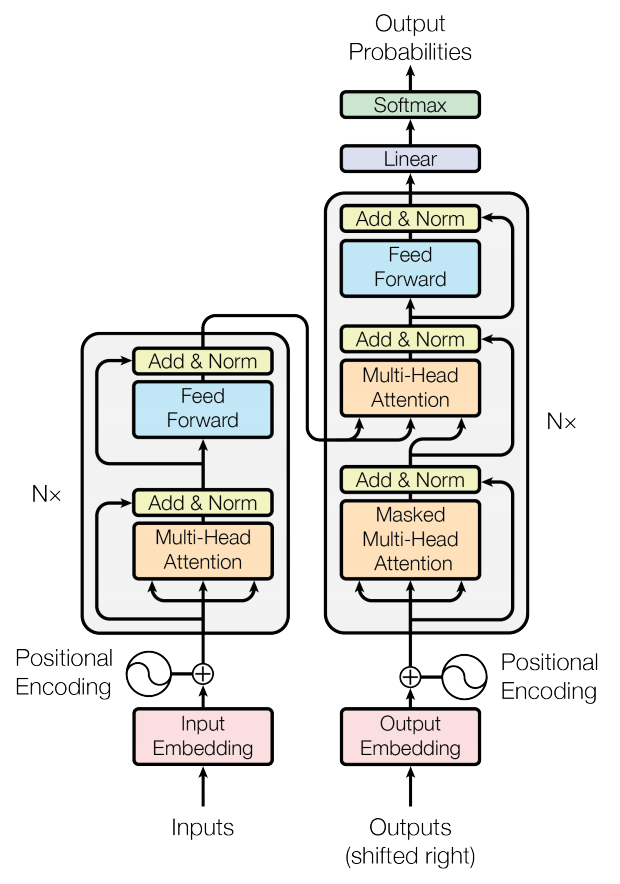
\includegraphics[width=10cm]{transformer}
	\caption{The Transformer model architecture (\cite{vaswani2017attention})}
	\centering
\end{figure}
The RNN encoder-decoder models have achieved state of the art in sequence modeling and machine translation problem. However such RNN models also have some disadvantages, because of their inherently sequential computation which prevents parallelization across elements of the input sequence. That means it is more difficult to fully take advantage of the modern computing devices like GPU and TPU. Convolutional \cite{gehring2017convolutional} and fully-attentional feed-forward architectures like Transformer \cite{vaswani2017attention} models are proposed as alternatives for RNNs. \\

%\textbf{Dot-Product Attention}
%Given a query $\bm{q}$ and a set of key-value $(\bm{k}-\bm{v})$ pairs, the output is weighted average of values, where the weight of each value is computed by inner product of query and corresponding key. The queries and keys are of the same dimension ${d_k}$, values are of dimension ${d_v}$. Actually, for better understanding, the query $\bm{q}$  can be considered as the decoder state $\bm{s}_i$ and key $\bm{k}$ and values $\bm{v}$ can be considered as the encoder state $\bm{h}_j$ in previous attention model. Then the attention of query $\bm{q}$ on all $(\bm{k}-\bm{v})$ pairs are:
%\[ A(\bm{q}, K, V) = \sum_{i}{ \frac{\exp\ ({\bm{q}\cdot \bm{k}_i})}{\sum_{j} \exp\ {\bm{q}\cdot \bm{k}_j} } \cdot \bm{v}_i}\]
%When we stack the queries ${\bm{q}}$ to ${Q}$:
%\[ A(Q, K, V) = \text{softmax}(QK^T)V\]
%
%As ${d_k}$ get larger, the variance of ${q^T k}$ get larger.  The softmax become very peaked and the gradient get smaller. To counteract this effect, we scaled the dot products by ${\frac{1}{\sqrt{d_k}}}$, we get
%
%\[ Attention(Q,K,V) = \text{softmax}(\frac{QK^T}{\sqrt{d_k}})V\]
%The shape of resulting matrix is $n_q \times d_v$\\
\textbf{Self-Attention}\\
\[ \alpha_{ki} = \frac{\exp(\text{score}(\bm{h}_k, \bm{h}_i))}{\sum_{j=1}^{I} \exp((\text{score}(\bm{h}_k, \bm{h}_j)))}\]
\[ \text{score}(\bm{h}_k, \bm{h}_i) = \bm{h}_k^\top \bm{h}_i /\sqrt{d} , \ \ \ d= \text{dim}(\bm{h}_k)\]
\[\bm{h}_k^{\prime} = \sum_{i=1}^{I} \alpha_{ki} \cdot \bm{h}_i\]

\textbf{Multi-head attention}\\
 First map $Q$, $K$, $V$ into $h$ many lower dimension spaces via linear mapping matrix. Here $h$ is the number of heads. Then apply attention and concatenate the outputs. \\
Suppose the original dimensions of queries, keys, values are ${d_{m}}$. We the number of heads is ${h}$, then we set ${d_k = d_v = d_{m}/h}$. With ${i \in 1 \cdots h}$ different matrix ${W_i^Q \in R^{d_{m}\times d_k}}$ ${W_i^K \in R^{d_{m}\times d_k}}$ ${W_i^V \in R^{d_{m}\times d_k}}$ and ${W^O \in R^{d_{m}\times d_k}}$.
The number of attention heads in Transformers impacts their ability to capture long-distance dependencies. Especially many-headed multi-head attention is essential for modeling long-distance phenomena with only self-attention.
\[ \text{MultiHead}(Q, K, V) = Concat(h\text{head}_1, \cdots, \text{head}_h)W^O \]
\[\text{head}_i = Attention(QW_i^Q, KW_i^K, VW_i^V) \]

where  $\text{head}_i \in \mathbb{R}^{n_q \times d_k}$,  ${\text{Multihead}(Q,K,V) \in \mathbb{R}^{n_q \times d_m}}$\\

\textbf{Encoder-Decoder Attention}
\[ \alpha_{ki} = \frac{\exp(\text{score}(\bm{s}_k, \bm{h}_i))}{\sum_{j=1}^{I} \exp((\text{score}(\bm{s}_k, \bm{f}_j)))}\]
\[ \text{score}(\bm{s}_k, \bm{h}_i) = \bm{s}_k^\top \bm{h}_i/\sqrt{d}, \ \ \ d= \text{dim}(\bm{s}_k)\]
%There are three attention types in the transformer model:
%\begin{itemize}
%	\item encoder-decoder attention\\
%	the queries come from the previous decoder layer, the keys and values are just the output of decoder. This works as the attention mechanism in the seq2seq model, it allow the decoder to align all positions in the input sequence with different weights
%	\item encoder self-attention\\
%	all queries, keys, values come from the encoder layer, each position allows to attend to all positions before that position
%	\item decoder self-attention\\
%	similar to encoder attention, each position is allowed to attend to position before and including that position
%\end{itemize}


\textbf{Positional Encoding}\\
Since there is no RNN or CNN structures in transformer model, we need also need to make use of sequence information for seq2seq learning. We need inject position information into the embedding.
\[PE_{(\text{pos}, 2i)} = sin(\text{pos}/ 10000 ^{2i / d_{m}})\]
\[ PE_{(\text{pos}, 2i+1)} = cos(\text{pos} / 10000^{2i/d_{m}})\]


where pos is the position and $i$ is the dimension. That is, each dimension of the positional encoding corresponding to a sinusoid.






\subsection{Neural Unsupervised Machine Translation}
 Although the neural machine translation systems have achieved near human-level performance on some languages, the lack of large parallel corpora poses a major challenge for many low-source languages.
 Techniques are raised to alleviate this issue with like triangulation and semi-supervised learning techniques.  Monolingual data are leveraged to improve the quality of translation system. \\
 Recently, several neural algorithms with fully unsupervised settings are proposed. The core ideal is very similar to the dual learning in machine translation. The systems all contain bi-directional models as sub-systems. Pseudo parallel data are created with back-translation. It turns the unsupervised problem into a supervised setting. As better translation , both sub-systems get improved synchronously.\\
 
%   the end-to-end method performs better and easier to tune without much specific linguistic knowledge. The Idea is similar to dual learning framework except that in dual learning model, gradients are backpropagated through the reverse model and pretrain using a relative large parallel data as a warm start. The neural model mapping the sentences from monolingual corpora into the same latent space, By learning to reconstruct in both languages from the shared feature space. The translation model in both direction will be improved synchronously with the back-translation.




%The key idea is to build a common latent space between the two languages (or domains) and to learn to translate by reconstructing in both domains according to two principles. 



%They initialize the model with an inferred bilingual dictionary. They leverage strong language model: denoising autoencoder,  third, they implemented the back translation: the key idea is to train two translation models which translate in contrary directions at the same time. The last property is that the models constrain the latent representations produced by the encoder to be shared between the two languages. The encoders will encoder the input into a common latent representation space independent of the language. The decoder plays the role of translator and will try to learn to improve the translation quality with the help of back translation mechanism.

\textbf{Dual Structure}\\
Dual structure is inspired by the observation: any machine translation has a dual task: e.g. German-to-English translation (primal) and English-to-German translation (dual). Dual tasks can form a closed loop and generate informative  feedback signals to for both translation models. Based on the feedback signals generated during this process, and leverage language model, we can minimize the reconstruction error of the original sentences. We can iteratively update the two models until convergence.   \cite{he2016dual} trained two agents to translate in opposite directions (e.g. French $\rightarrow$ English and English $\rightarrow$ French), and make them teach each other through a reinforcement learning process. While promising, this approach still requires a parallel corpus for a warm start. \cite{lample2018phrase} simplified the structure, in the proposed model, the gradients will not be back-propagated through the reverse model, but only make use of the back-translation. The training process as followed:\\

\begin{algorithm}[H]
	\SetAlgoLined
	\textbf{Language models:} Learn language models $P_s$, $P_t$ over source and target languages;\\
	\textbf{Initial translation model:}  Leveraging $P_s$, $P_t$, lean two initial translation models in each direction: $P_{s\rightarrow t}^{(0)}$, ${P_{t \rightarrow s}^{(0)}}$;\\
	\For{k = 1 to N}{
		\textbf{Back-translation:} Generate source and target sentences using the current translation models $P_{t\rightarrow s}^{(k-1)}$ and $P_{s\rightarrow t}^{(k-1)}$, leverading $P_s$, $P_t$;\\
		\textbf{Retrain:} Train new translation models $P_{t\rightarrow s}^{(k)}$ and $P_{s\rightarrow t}^{(k)}$ using the generated sentences and leverading $P_s$, $P_t$;
	}
	\caption{Unsupervised Machine Translation}
\end{algorithm}


\textbf{Initialization}\\
Without enough information to start the dual machine translation system, it will be hard for the system to catch the meaningful signals and then it will take much more iterations. However if we initialize the system by a naive a word-by-word translation of the sentence, where the bilingual lexicon are derived from the same monolingual data. Though such initial "word-by-word" translation maybe poor if languages or corpora are not closely related, it still preserves some  original semantics. Such word-by-word translation can actually achieve several BLEU scores.\\
%\log P_{t\rightarrow t}(e|\text{noise}(e)
%\log P_{s\rightarrow s}(f|\text{noise}(f)) 


\textbf{Shared Latent Representation} \\
A shared encoder representation actis like an interlingua, which is translated in the decoder corresponding language regardless less of the input source language. Since the only supervision information only comes from the monolingual data. The model learn to translate by learning to reconstruct in both language from this shared space.\\
There are two different methods to learn the shared feature space:
\begin{itemize}
	\item Shared encoder
	The system use only one encoder that is shared by both languages involved. The universal encoder is aimed to produce a language independent representation of the input language but the decoder should separately translate then into corresponding language.
	\item Adversarial training
	Train discriminator to classify between the encoding of source and target sentences. The discriminator operates on the output of the encoder, the encoder is trained instead to fool the discriminator. 
\end{itemize}



\textbf{Optimization}\\
When minimizing the loss function, gradients will not be back propagated through the reverse model which generate the data. Instead the objective function minimized at every iteration is the sum of $L^{auto}$ and $L^{back}$
\begin{itemize}
	\item Denoising autoencoder loss
	\[ L^{auto} = \mathbb{E}_{\bm{e}\sim E}[-\log P_{t\rightarrow t}(\bm{e}|\text{noise}(\bm{e})] + \mathbb{E}_{\bm{f}\sim F} [-\log P_{s\rightarrow s}(\bm{f}|\text{noise}(\bm{f}))]\]
	where $s$ $P_{s\rightarrow s}$ and $P_{t\rightarrow t}$ are the composition of encoder and decoder both operating in the source and target sides, respectively
	\item Back-translation loss
	\[ L^{back} = \mathbb{E}_{\bm{e}\sim T} [-\log P_{s\rightarrow t}(\bm{e}|u(\bm{e}))] +  \mathbb{E}_{\bm{f}\sim S} [-\log P_{t\rightarrow s}(\bm{f}|v(\bm{f}))]\]
	 we denote the sentence that translated by intermediate target-to-source translation model as $u(y)$, similarly denote the sentence translated by source-to-target model as $v(x)$, so $u(y)$ should in source language and $v(x)$ should in target language. The pairs $(x, v(x))$, $(u(y), y)$ constitute synthetic parallel  sentences.
\end{itemize}

\begin{figure}[H]
	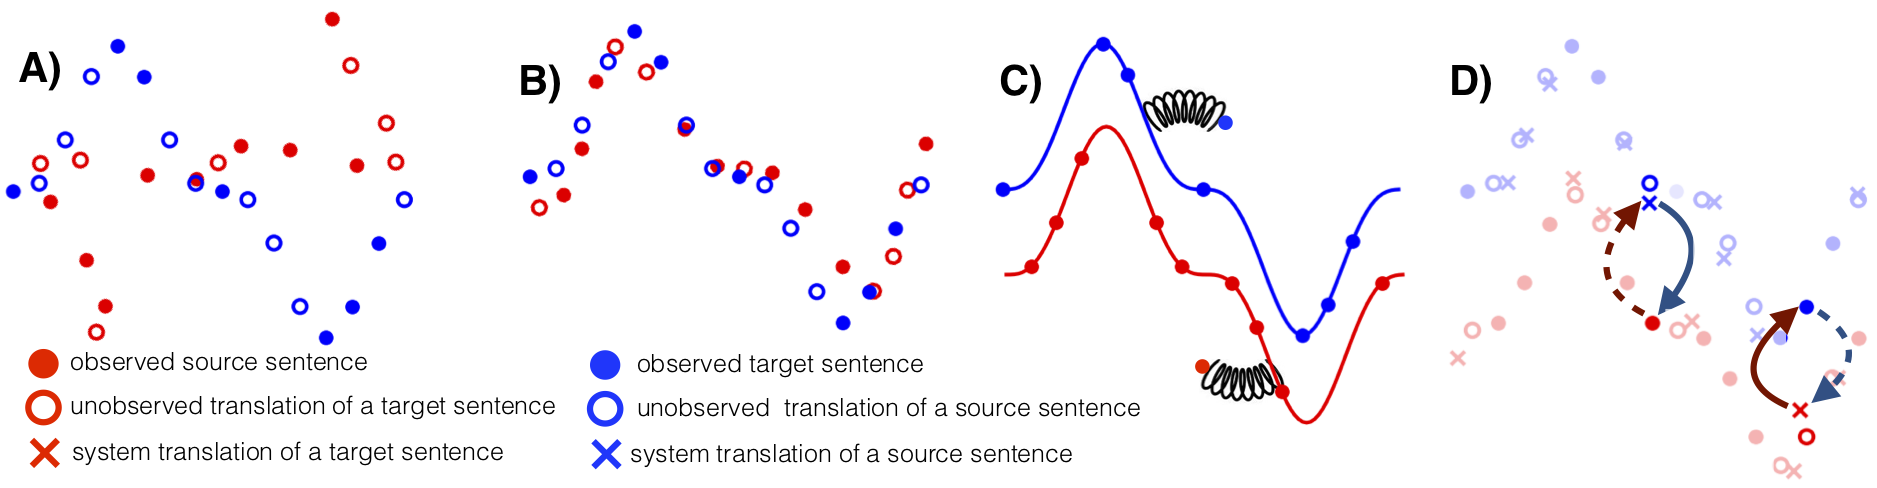
\includegraphics[width=14cm]{unmt}
	\caption{Key techniques for neural unsupervised machine translation: A) the two original monolingual data; B) Initialization, the two distribution are roughly aligned; C) Denoising autoencoder, make the distribution closer to normal one in corresponding language D) Back-translation, improve the both translation model in iterative way (\cite{lample2018phrase})}
	
\end{figure}











\glsresetall
\chapter{Word Embedding}
%Word embeddings is distributed representation of words in a vector space. With the learning algorithm it can capture the contextual or co-occurrence information. The word embedding has an interesting and important property: similar words will have similar distribution in the embedding space, with that property, we can find meaningful near-synonyms or  Some successful methods for learning word embedding like word2vec\cite{mikolov2013distributed}, \cite{pennington2014glove}
%Word embeddings, when used as the underlying input representation, have been shown to boost the performance in  neural network models for natural language processing (NLP) tasks such as sequence tagging and text classification.
Researchers have worked on a number of methods for using word embedding in MT tasks. It has been proven that word embedding helps to improve the translation quality and handle the Out-Of-Vocabulary (OOV) problems (\cite{neishi2017bag}, \cite{qi2018and}). Recently, cross-lingual word embedding is quickly gaining in popularity. They play a crucial role in transferring knowledge from one language to another. Cross-lingual word embeddings have been used either in standard machine translation system (\cite{lample2017unsupervised}) or as a method for learning translation lexicons in an entirely unsupervised manner (\cite{xing2015normalized}, \cite{lample2018phrase}). \\
%\cite{neishi2017bag} attempt initializing the embedding layers with pre-trained word embeddings on the training datasets in the source languages. They find such method can improve the translation quality.  \cite{qi2018and} point that pretrained embeddings seem to be more effective for more similar translation pairs and it helps most when the training data is not large enough. Word embedding are also exploited to handle the out-of-vocabulary (OOV) problem.\\
Before we discuss the cross-lingual word embedding in this chapter, I will first introduce the learning algorithm for monolingual word embedding.Then I will explain the training and the lexical translation inference methods.

\section{Monolingual Embedding}
%A large majority of cross-lingual embedding models take inspiration from and extend monolingual word embedding models to bilingual settings, or explicitly leverage monolingually trained models. As an important preliminary, we thus briefly introduce monolingual embedding models.
Word embedding is distributed representation of word in high dimensional space. It can capture the contextual or co-occurrence information, so that similar words have similar distribution in the embedding space.  Several methods have been proven to be success like word2vec (\cite{mikolov2013efficient}) GloVe (\cite{pennington2014glove})
\begin{figure}[h]
	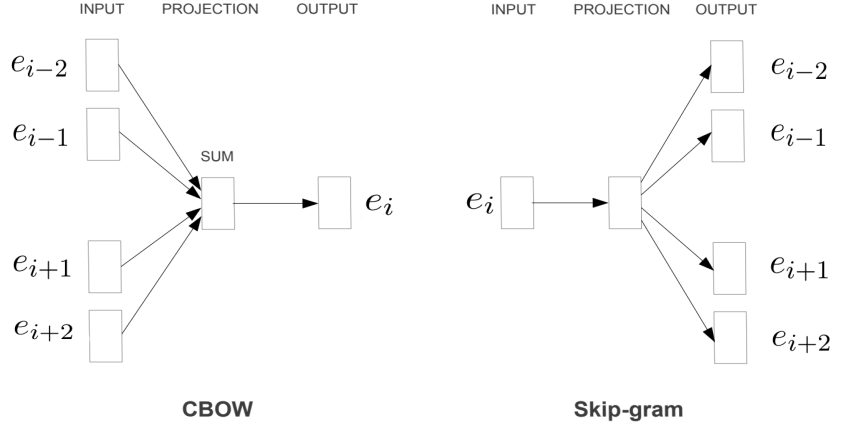
\includegraphics[width=12cm]{skip}
	\caption{Global attention model (\cite{mikolov2013efficient})}
	\centering
\end{figure}
\subsection{CBOW and Skip-gram}
CBOW and skip-gram are current mainstream neural network model to learn word embedding. Algorithmically,  CBOW tries to predict the current word based on the context while skip-gram model is to find better representations that are useful for predict \cite{qi2018and}ing the context words. Using skip-gram model as example, given a large training corpus represented as a sequence of words ${e_1^N: = e_1, \cdots e_I}$, the objective of the model is to maximize the following log-likelihood:
\[ \mathcal{L}^e_{\text{skip-gram}} = - \frac{1}{I} \sum_{i=1}^{I} \sum_{ -c \le d \le c, d\ne 0} \log\ {p(e_{i+d}|e_i)}\]

where $e_i$ is the current word and $c$ is the size of training context. \\


Similarly, we define the loss for CBOW model as
\[ \mathcal{L}^e_{\text{CBOW}} = - \frac{1}{I} \sum_{i=1}^{I} \sum_{ -c \le d \le c, d\ne 0} \log\ {p(e_{i}|e_{i+d})}\]

\textbf{Negtive Sampling}\\
The prediction probability $p(e_{i+d}|e_i)$ is defined as a softmax function:
\[p(e_{i+d}|e_i) = \frac{\exp \{ \text{score}(e_{i+d},e_i)\} }{\sum_{e^{\prime} \in V_e}{\exp  \{ \text{score}(e^{\prime}, e) \}}}\]
where $V_e$ is the entire vocabulary. 
The normalization over $V_e$ is very expensive since it is calculate for all words at every training steo. Negative sampling is proposed to approximate the sofrmax to make it computationally more efficient. It trains to model to distinguish a target word from negative samples drawn from a noise distribution \text{noise}.
\[p(e_{i+d}|e_i) = \log p(e_{i+d}=1| e_i) + \frac{1}{k} \sum_{e^{\prime} \in p_{\text{noise}}}\log p(e^{\prime}=0|e_i)\]
where $p(\cdot| e_i)$ is a model to predict if the word is in the context of $e_i$.\\ 
\textbf{Subword Information}\\
The training methods mentioned treat each word as a distinct word embedding, however, intuitively we can obtain more information from the morphological information of words. A subword model is proposed to capture the subword informaion. The training network is still CBOW or skip-gram. Each word is represented as a bag of character-level $n$-grams and assign a distinct embedding for each character $n$-gram. Score function in the network is calculated using the sum of inner products of the subword embeddings (\cite{DBLP:journals/corr/BojanowskiGJM16}). 
\subsection{GloVe}
Global vectors(GloVe) allows us to learn word representations via matrix factorization. GloVe minimizes the difference between the dot product of the embeddings of word and its context and the logarithm of their number of co-occurrences within a certain window size:
\[ \mathcal{L}_{GloVe}^e = \sum_{i,j=1}^{\lvert V_e \rvert} f(C_{ij})({\bm{e}_i}^{\top} \bm{e}_j - \log{C_{ij}} ) \]
where the matrix of word-word co-occurrence counts be denoted as $C$, whose entries $C_{ij}$ tabulate the number of times word $e_j$ occurs in the context of word $e_j$ and $f(\cdot)$ is a weighting function that assigns relatively lower weight to rare and frequent co-occurrences. $V_e$ is the source vocabulary size.
%Furthermore in skip-gram model, suppose given a scoring function s which maps word pairs to score in $\mathbb{R}0$ like cosine similarity, the probability can be defined as
%\[ p(e_{i+j} | e_i)  = \frac{\exp\{s(e_{i+j}, e_j)\}}{\sum_{e^{\prime} \in V^e }{\exp\{s( e^{\prime}, e_i)\}}}\]
%where $V^e$ is the whole vocabulary. \\
%
%\textbf{Negative Sampling}\\
%However the normalization on the whole vocabulary is very expensive since it is conducted for all words at every training step. Negative sampling is proposed to approximate the softmax to make it computationally more efficient. The problem of predicting words can be considered as an independent binary classification task. Negative sampling trains the model to distinguish a target word from negative samples drawn from a noise  distribution $P_{\text{noise}}$.   
%\[p(e_{i+j}|e_i) = \log {Q_{\theta}{(D=1 | e_{i+j}, e_i)}} + \frac{1}{k}\sum_{e^{\prime} \sim P_{\text{noise}}} {\log{Q_{\theta}{(D=0 | e^{\prime}, e_i )}}}  \]
%
%where ${Q_{\theta}{(D=1| w_t, w_s)}}$ is the binary logistic regression probability.
%According to  empirical results, CBOW works better on smaller datasets because CBOW smoothes over a lot of the distributional information while Skip-Gram model performs better when we have larger datasets
%
%\subsection{Enriching Embedding with Subword Information}
%The training methods above treat each word as a distinct word embedding, however intuitively we can obtain more information from the morphological information of words. A subword model was proposed to try to fix such problem.The training network is similar, the model design a new presentation of the word: it adds speicial symbols $<$, ${>}$ as boundary information at the beginning and the end of a word. Then a normal word is represented as a bag of character $n$-grams . For example the word "where" and n equals 3, the it can be represented as the following 5 tri-grams: 
%\[ <wh, whe, her, ere, re>\]
%Suppose in this way for a specific word $e$ ${G_{e}}$ the set of character ${n}$-grams, we assign for each character ${n}$-gram $g$ in ${G_{e}}$ a distinct vector $\bm{v}_g$, we calculate the score function using the sum of character-level inner product of vectors:
%\[s(e^{\prime}, e) = \sum_{g \in G_{e}} \bm{v}_g^{T} \bm{e}^{\prime} \]
%where $\bm{e}^{\prime}$ the embedding of $e^{\prime}$
\section{ Cross-lingual Word Embedding}
% NLP tasks in multilingual scenarios is receiving increasing interest. The need to represent meaning and transfer knowledge in cross-lingual applications has motivated the work on cross-lingual models, which learns the representations in a joint embedding space.
  \cite{mikolov2013exploiting}  observe that word embeddings trained separately on monolingual corpora exhibit isomorphic structure across languages, as illustrated in Figure $3.2$. That means we can create a connection between source embedding and target embedding even with simple linear mapping. This has far-reaching implication on low-resource scenarios (\cite{adams2017cross}), because word embedding training requires only plain text to train, which is the most abundant form of linguistic resource.
\begin{figure}[t]
	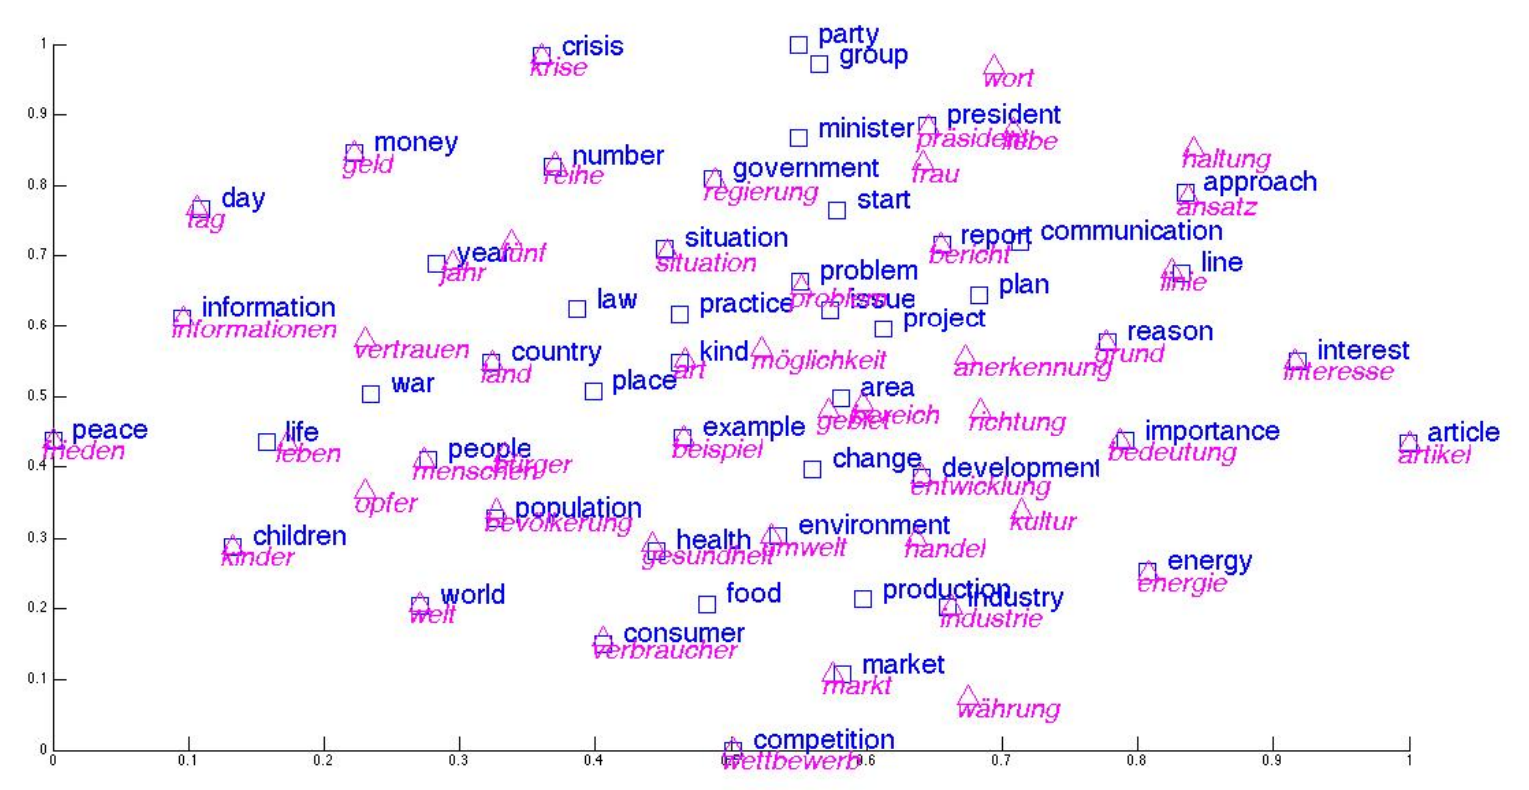
\includegraphics[width=14cm]{crossembedding}
	\centering
	\caption{A cross-lingual embedding space between German and English (\cite{ruder2017survey})}
\end{figure}

%In the thesis, I assume there are two set of embeddings ${e}$, ${f}$trained separately on monolingual data.  The propose of cross-lingual word embedding training is to learn such a mapping ${W \in }$ from source embedding space to target embedding space, so $Wf_i, e_j$ in the same embedding space and for all corresponding word pairs, we need to optimize the mapping ${W}$, so that"
%
%
%\[ \arg\min_{W \in R^{d \times d}} \sum_{i} \lVert Wf_i - e_i \rVert \]
%where $d$ is the dimension of embeddings, and the distance ${\lVert Wf_i - e_i \rVert}$ can be different types. We prefer the Euclidean distance.  
%
%first
	

\subsection{Supervised Training}
Before we go on to the main training setting of this thesis (unsupervised), I will introduce the training methods under supervision. The supervision comes from seed lexicons, parallel data or document-aligned data.\\
Supervised training methods of cross-lingual word embedding can be divided into joint training approaches and mapping-based approaches. The difference is that joint methods train directly the cross-lingual word embeddings, while the mapping-based approaches first train monolingual word representations on corresponding corpus separately. Then mapping will be learned to project different embeddings into a shared space according to supervision signals. \\

\textbf{Joint Training Approaches}\\
Here the joint training means to optimize source and target embedding objectives $\mathcal{L(\cdot)}$ together with the cross-lingual regularization term $\Omega(\cdot)$. 
\[ \mathcal{L} =  \mathcal{L}_{\text{mono}}^e + \mathcal{L}_{\text{mono}}^f + \cdot \Omega(\cdot)  \]
where the first two losses are exact the same as those in monolingual embedding training.  $\Omega(\cdot)$  encourages representations to be similar for words that are related across different languages.

Different cross-lingual regularization terms are proposed to optimize the cross-lingual embeddings (\cite{coulmance2016trans}, \cite{luong2015bilingual}, \cite{gouws2015bilbowa}). For example, \cite{gouws2015bilbowa} models it as: 
\[ \Omega_{\text{BilBOWA}} = \sum_{( f_1^J, e_1^I)}{\lVert \frac{1}{I}  \sum_{e_i \in e_1^I} \bm{e}_i - \frac{1}{J} \sum_{f_j \in f_1^J} \bm{f}_j\rVert}^2 \]
where $\bm{f}_j$ and $\bm{e}_i$ are the word embeddings for words in parallel source and target sentences $(f_1^J, e_1^I)$. Instead of relying on expensive word alignments which minimize the distance that aligned to each other, they minimize the distance between the mean of the word representations in the aligned sentences. \\

\textbf{Mapping-based Approaches}\\
Another approach is to train monolingual word representations separately on monolingual corpora and then learn a transformation matrix mapping that maps representations in one language to the representations of other language.  This approach can be further divided into learning separate mappings for each language or learning mapping only for source language to project source embeddings into target embedding space.

learn the transformation for each language, both monolingual embeddings are mapped into a shared embedding space. The typical model is CCA-based approaches (\cite{faruqui2014improving}, \cite{dhillon2011multi} and \cite{lu2015deep}). The other method is to learn the mapping from the source embedding space to the target embedding space. The criterion is to minimize the mean squared error between the transformed source embeddings and the target embeddings. The advantage of this method is that it is really fast to learn the embeddings and embedding alignments. People criticize whether linear or nonlinear can capture the relationship between all words in different languages.
\begin{itemize}
	\item Mapping matrix for each language\\
	The typical method is  canonical correlation analysis(CCA).
	\begin{figure}[t]
		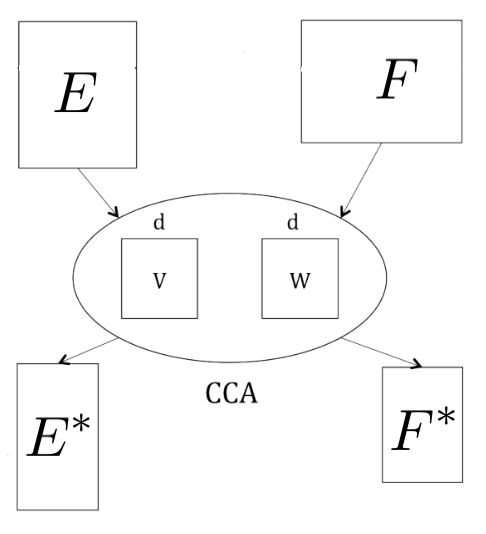
\includegraphics[width=8cm]{cca}
		\centering
		\caption{Cross-lingual projection with CCA (\cite{faruqui2014improving})}
	\end{figure}
	let $F $ and $E$ be the embedding matrices comprised of seed word translation pairs. The  $W$ and $V$ are the projection matrices which mapped the original embedding matrices into $F^{*}$ and $E^{*}$, which are in the joint space, $d$ is the embedding dimension.
	
	\[ {F}^{*} = W{F} \ \ \ \  {E}^{*} = V{E} \] 
	The objective of CCA is to find the two matrices such that the projections of the parallel matrices are maximally correlated:
	\begin{align}
		W^*, V^* =& \argmax{W, V \in \mathbb{R}^{d \times d}} \text{corr}(WF, VE)\\
		= &\argmax{W, V \in \mathbb{R}^{d \times d}} \frac{\mathbb{E}[(W{F})(V{E})]}{\sqrt{\mathbb{E}[(W{F})^2]} \sqrt{\mathbb{E}[( V{E})^2]}}
	\end{align}

	Once we get the two projection matrices, we can calculate the cross-lingual word embedding for the entire source and target vocabulary.
	
	A linear feature mapping is often not sufficiently powerful to faithfully capture the hidden, non-linear relations within the data. \cite{lu2015deep} propose a non-linear extension of CCA using deep neural networks to maximize the
	correlation between the projections of both monolingual embedding spaces
	\[ f_1^*, f_2^* = \argmax{f_1, f_2} \ \text{corr}(f_1(F), f_2(E)) \]
	where $f_1$ and $f_2$ are non-linear transformation implemented by neural networks.
	
	\item Mapping matrix for only source language
	\cite{mikolov2013exploiting} notice that the geometric relation that hold between words are similar across languages. This suggest that, we can learn the transformation directly from source embedding space to target space.
	Given a seed word translation pair set $dico$, the objective is to learn $W$ that minimizes the distance between mapped source word embedding $W\bm{f}$ and corresponding target embedding $\bm{e}$:
	\[ \argmin{W} \sum_{(\bm{f}, \bm{e}) \in dico}  {\lVert W\bm{f} - \bm{e} \rVert}_2^2 \]
	This can also be expressed in matrix form as minimizing the squared Frobenius norm of the residual matrix $F$, $E$:
	\[ \argmin{W} {\ \lVert WF - E \rVert}_{\text{F}}^2 \]
	
	
	
	\cite{xing2015normalized} showed that the results are improved when we use $l_2$ normalized embeddings and constrain the ${W}$ to be an orthogonal matrix. In this case we can use Procrustes analysis which advantageously offers a closed form solution obtained from the singular value decomposition 
	\[W^* = \argmin{W \in O_d(\mathbb{R})} {\ \lVert WF - E \rVert}_{\text{F}}^2 = UV^T , \quad U\Sigma V^T = \text{SVD}(EF^T) \]
	where $ O_d(\mathbb{R})$ denotes manifold of orthogonal matrices 
\end{itemize}


\[ \]
%where $W_f$ and $W_e$ are the weights of the two networks and ${}$ ${}$, ${}$ are covariance matrices computed for   in the ssame way as CCA. The final transformation is the composition of the neural network ans CCA projection, $\bm{u}^T \bm{f}$ for the view. The algorithm does not have a closed-form solution but the parameters can be learned via gradient-based optimization with mini-batch stochastic gradient descent .
%\begin{enumerate}
%	\item Mapping based approaches\\
%	First train the monolingual word embedding separately and then seek the seed dictionary to learn the mapping. 
%	\item Pseudo-multi-lingual corpora-based approaches\\
%	Use the monolingual embedding training method on constructed corpora that contains both the source and the target language.
%	\item Joint methods\\
%	Take the parallel text as input and minimize the source and target language losses jointly with the cross-lingual regularization term
%\end{enumerate}





%In order to make learning and inference consistent, \cite{DBLP:journals/corr/abs-1804-07745} propose the relaxed CSLS loss (RCSLS), which is inspired from the work of \cite{conneau2017word}
%
%The loss function can be rewritten as:
%\[ \min_{\bm{W} \in \mathcal{O}_d} = \frac{1}{n} \sum_{i=1}^{n} \Big\{ -2 \bm{f}_i^\top W^\top \bm{e}_i + \frac{1}{k} \sum_{\bm{e}_j \in \mathcal{N}_e(W\bm{f}_i)} \bm{f}_i^\top W^\top \bm{e}^j + \frac{1}{k} \sum_{W\bm{f}_j \in \mathcal{N}_f(\bm{e}_i)} \bm{f}_j^\top W^\top \bm{e}^i  \Big\}\]

%
%Normally, the size $n$ of the dictionary is too small with respect to the entire vocabulary size, in order to incorporate unlabeled data, the unpaired words in the dictionary are used as "negatives samples" in the RCSLS loss, as result, we can optimize the loss function not only the dictionary but the whole vocabulary.

\subsection{Biligual Lexicon Induction}
When we use nearest neighbors search to infer the word translation, we suffer from the so-called "hubness Problem": points are tending to be nearest neighbors of many points in high-dimensional space.  Those points (hubs) will harm the search accuracy.\\
Now this limitation is addressed by apply a applying a corrective metric at inference time, such as inverted softmax (ISF)(\cite{smith2017offline})  or cross-domain similarity scaling (CSLS)(\cite{conneau2017word})
\begin{itemize}
	\item Inverted Softmax (ISF)\\
	The confidence of choosing a target word as translation of a source word can be considered as softmax-like normalized probability
	\[ p(e|f) = \frac{\exp{\Big(\beta \cdot  \text{score}(e,f)\Big)}}{\sum_{e^{\prime}} {\exp{\Big(\beta \cdot \text{score}(e^{\prime}, f)\Big)}}} \]
	where the $\text{score}(\cdot)$ is the score function we can define ourselves.
	we learn the "temperature" $\beta$ by maximizing the log probability over the training dictionary. 
	\[ \argmax{\beta} \sum_{e,f} \ln p(e|f)  \]
	
	The author observed that, if we invert the softmax and normalizing the probability over all the source words rather than target words, the hubness problem could be mitigated:
	\[ p(e|f) = \frac{\exp{\Big(\beta \cdot  \text{score}(e,f)\Big)}}{\alpha \  \sum_{f^{\prime}} {\exp{\Big(\beta \cdot \text{score}(e, f^{\prime})\Big)}}}\]
	\item  Cross-domain Similarity Local Scaling (CSLS)\\
	We denote ${\mathcal{N}_e(\bm{f})}$ the set of ${k}$ nearest neighbors of points of the mapped $\bm{f}$ in the target embeddiWe use the phrase embedding also in the machine translationng space, and ${\mathcal{N}_f(\bm{e})}$ the nearest neighbors of mapped ${\bm{e}}$ in the source embedding space. We consider the mean cosine similarity as hub-ness:
	\[ r(\bm{f})= \frac{1}{K} \sum_{\bm{e}^{\prime} \in \mathcal{N}_e(\bm{f})} \cos(\bm{e}^{\prime}, W\bm{f})\]
	So in this way we penalize the hub points:
	\[ CSLS(\bm{e}, \bm{f}) = 2 \cos(\bm{e}, \bm{f}) - \frac{1}{k} \sum_{\bm{e^{\prime}} \in \mathcal{N}_e(\bm{f})} \cos(\bm{f}, \bm{e^{\prime}})- \frac{1}{k} \sum_{\bm{f^{\prime}} \in \mathcal{N}_f(\bm{e})} cos(\bm{f^{\prime}}, \bm{e}) \]
\end{itemize}


%Since we use the pseudo parallel data (source sentence and word-by-word target translation sentence), we can exploit the context information from language model to select the word translation candidate. Beam search with language model is implemented here. More details about sentence translation will be explained next chapter.\\
\section{Phrase Embedding}
Different methods are proposed to learn phrase embedding, which can be mainly divided into two categories. The first is based on the distributional hypothesis; it treats a phrase as fundamental unit as that in phrase-based MT. Phrases will be considered as non-divisible and phrase embedding algorithm is similar to word embedding. However, distributional methods cannot make use of the information embedded in component words and they also face data spareness problem. The second is based on the principle of compositionality. It infers phrase embedding according to the embeddings of its component words. However,  many phrases have a meaning that is not simple composition of the meaning of its individual words. \\
In this paper, we follow first idea, we train the phrase embeddings using the data-driven method proposed by \cite{mikolov2013distributed}. We also propose a novel phrase detection method. We find that our method is easy to implement and to tune the parameter. In experiments, our method works obviously better than the other one with the same phrase skip-gram training.\\

\textbf{Phrase Detection}
\begin{itemize}
	\item Phrases formed based on the unigram and bigram counts (\cite{mikolov2013distributed})\\
	\[\text{score}(e^{\prime}, e) = \frac{\text{count}(e^{\prime}, e)-\delta}{\text{count}(e^{\prime}) * \text{count}(e)} \]
	where $\delta$ is a discounting coefficient and prevents too many phrases consisting of very infrequent words to be formed. The bigrams with score above the chosen threshold are then used as
	phrases. 
	\item Process sentences with most common phrases in training corpus\\
	We count the most frequent bigrams in training corpus, using the counts directly as phrase score: $\text{score}(e^{\prime}, e) = \text{count}(e^{\prime}, e)$. We maximize the sum of phrase scores in given sentences in order to detect the phrases with dynamic programming. In our approach we consider the top-$k$ as the only parameter.
\end{itemize}

With the same training algorithm as word embedding, we can obtain the phrase embeddings. We use the phrase embeddings also in the machine translation system, which will be explained in Chapter 5, and find phrase embeddings performs better than word embedding iunder some specific settings. Experiment results are demonstrated in Chapter 6.4.4.

\glsresetall
\chapter{Unsupervised Learning of Cross-lingual Word Embedding}
Chapter 3 introduces the supervised learning of cross-lingual word embedding, they employ parallel data like bilingual dictionary or parallel corpora and have shown strong results on a word retrieval task.  However, labeling the lexicon information still costs lots of labor. This motivates people to explore fully unsupervised method. In this chapter, several unsupervised approaches will be explained including a novel corpus-based approach, which is distinct from other methods by exploiting an extra language model and corpus-based training process. All these approaches contains an iterative training procedure. 
\section{Initialization}
Pre-trained monolingual embeddings capture distribution information for each language. These embeddings are typically not expected to be aligned between languages A good initialization is a key to the iterative training framework.
A practical approach for reducing the need of bilingual supervision is to design heuristics to build the seed dictionary. \cite{hauer2017bootstrapping} propose to use shared words and cognates to extract the seed dictionary. This method has a flaw that it depends on the writing system. \cite{artetxe2018robust} raise a method that using similarity matrix to capture rough cross-lingual signals.\\

\subsection{Heuristics}
The seed is constructed by identifying words with similar spelling (cognates). A relative-frequency constraint is imposed to filter out word pairs that have fully different meaning; generate the list of words by frequency first, for each source word, if there exists target word that the normalized edit distance (NED) and absolute difference between the respective frequency ranks is within a specific threshold, these two word will be added into a seed dictionary.  This noisy seed lexicon will be considered as initial signals. There is no one-to-one constraint, so both source and target words may appear multiple times in the seed. 

\subsection{Similarity Matrix}
Similarity matrix is based on a simple assumption: while the axes of the original ${\lvert \tilde{V} \rvert}$ most frequent embeddings ${F \in \mathbb{R}^{d \times {\lvert \tilde{V} \rvert} }}$ and ${E \in \mathbb{R}^{d \times {\lvert \tilde{V} \rvert} }}$  are different, but $M_F=F^{\top}F$, $M_E = E^{\top}E$ capture the similarity inner respective languages. The similarity matrices $M_F$ and $M_E$ would be equivalent up to a permutation of their rows and columns. For example, in one language, the similarity between $a,b,c$ and $i,j,k$ is as the left graph in Figure 4.1, suppose ideal the their corresponding translations are $a^{\prime},b{\prime},c{\prime}$ and $i{\prime},j{\prime},k{\prime}$, but the order differs as the middle graph. If we first sort the values in each row, it will be much easier to find the relationship between $a$ and $a^{\prime}$, etc.. They find $\sqrt{M_F}$ and $\sqrt{M_E}$ 
work better in practice.
\begin{figure}[H]
	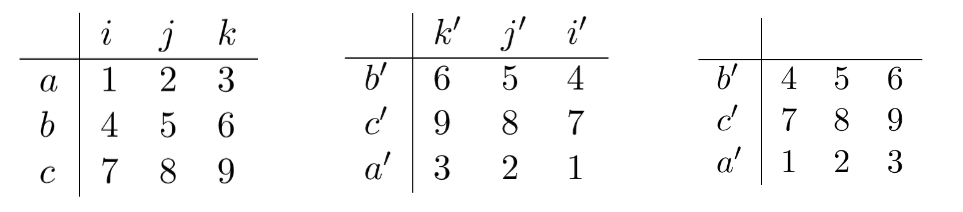
\includegraphics[width=12cm]{similarity}
	\centering
	\caption{Illustration of similarity matrix method}
\end{figure}

While the latter is far from the accurate alignment, it works well as the initialization for the iterative methods described next.
\section{Vocabulary-based Learning}
The vocabulary-based approach depends on high-quality lexical information to learn the mapping between embedding distributions.
We can use Figure 4.2 to illustrate the vocabulary-based learning process. As in graph (A) there are two distributions of word embeddings, source words in red denoted by $F$ and target words in bleu denoted by $E$, which we want to align. Each dot represents a word in shared space. Using initialization, we learn a rotate matrix $W$ which roughly aligns the two distributions. According to dictionary induction, we can find some reliable points in graph (B). We can futher refine the mapping $W$, using frequent words aligned by the previous step as anchor points, and minimizes a loss function measured by mapping distance as in graph (C). Repeat steps in (B) and (C), we hope to find a liner mapping that can be generalized to all words in the dictionary as in graph (D).
\begin{figure}[H]
	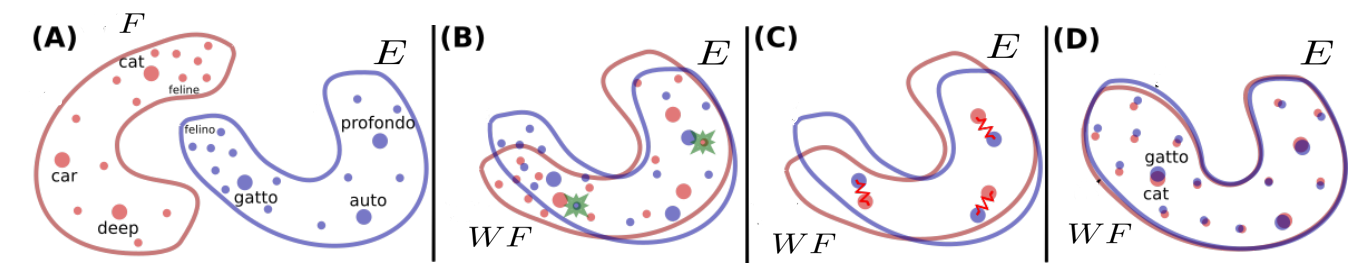
\includegraphics[width=12cm]{vocab}
	\centering
	\caption{Illustration of vocabulary-based learning (\cite{conneau2017word})}
\end{figure}
\subsection{Iterative Procrustes Analysis}
After initialization, the words in the seed dictionary can be considered as temporary  anchor points for Procrustes analysis, which has been introduced in Section 3.2.1.
Apply the Procrustes solution on the current seed dictionary, use the learned mapping matrix $W$ and dictionary induction technique to construct a better seed dictionary again. Repeat such process we suppose to obtain a hopefully better mapping and dictionary until some convergence criterion is met. The training will be stopped when the improvement on the average dot product for the induced dictionary falls below a give threshold from one iteration to the next. In practice, the threshold value is set at $1e-6$.  To prevent the mapping and dictionary from getting stuck in local optima, Mutual nearest neighbors and thresholding are used to ensure a high-quality dictionary. In the experiments we find that intersection of two unidirectional dictionaries work better than union or a unidirectional dictionary,  that is to say, the quality of dictionary plays more important role than the quantity.\\
\begin{figure}[h]
	\centering
	\begin{minipage}{.7\linewidth}
		\begin{algorithm}[H]
			\SetAlgoLined
			\KwIn{$F$ (source embeddings)}
			\KwIn{$E$ (target embeddings)}
			\KwIn{$dico$ (seed dictionary)}
			\KwResult{$W$ (embedding mapping) }
			\While{not converge}{
				${W \leftarrow LEARN\_MAPPING(F,E,dico)}$
				${dico \leftarrow LEARN\_DICTIONARY(W)}$
				
			}
			\caption{Iterative training procedure}
		\end{algorithm}
	\end{minipage}
\end{figure}

\subsection{Adversarial Training (GANs)}
The adversarial training was for cross-lingual embedding mapping is first proposed by \cite{barone2016towards}, who combines an encoder that maps source word embeddings into the target embedding space, a decoder that reconstructs the source embeddings from the mapped embeddings and a discriminator that discriminates between embeddings. \cite{zhang2017adversarial} incorporate additional techniques like noise injections to aid the training. \cite{conneau2017word} finally achieve good results by dropping the reconstruction component regularizing the mapping to be orthogonal\\
Let ${=\{ \bm{f}_1, \cdots, \bm{f}_{{\lvert \tilde{V} \rvert}}\}}$ and ${ = \{ \bm{e}_1, \cdots , \bm{e}_{{\lvert \tilde{V} \rvert}}\}}$ be the most ${\lvert \tilde{V} \rvert}$ frequent word embeddings from source and target languages respectively. We refer the discriminator parameters as ${\theta_D}$.The discriminator is a multi-layer neural network trained to discriminate the transformed source word embedding from the target word embedding, while the mapping $W$, as simple as a linear transformation, is trained to fooling discriminator. In the two-player game, mapping from source embedding space to the target space is supposed to be learned.\\

Generator loss 
\[ \mathcal{L_G}(W|\theta_D) =  -\frac{1}{{\lvert \tilde{V} \rvert}} \sum_{n=1}^{\tilde{V}}\log P_{\theta_D}(source=0|W \bm{f}_n) - \frac{1}{\tilde{V}} \sum_{n=1}^{{\lvert \tilde{V} \rvert}} \log P_{\theta_D}(source = 1 | \bm{e}_n) \]
Discriminator loss
\[ \mathcal{L_D}(\theta_D | W) =  -\frac{1}{{\lvert \tilde{V} \rvert}} \sum_{n=1}^{{\lvert \tilde{V} \rvert}} \log P_{\theta_D}(source = 1| W\bm{f}_n) - \frac{1}{{\lvert \tilde{V} \rvert}} \sum_{n=1}^{{\lvert \tilde{V} \rvert}} \log P_{\theta_D}(source=0| \bm{e}_n) \]	 
\section{Corpus-based Learning}
\subsection{Motivation}
The vocabulary-based training approach makes good use of the  embedding distribution similarity. However, it just looks at the mutual nearest neighbors, not considering polysemy of the words.  It does not take the semantic or contextual information into consideration when training the cross-lingual mapping, which would be a flaw especially in machine translation task. We also argue that word frequency should also be considered when training. For example, though words are synonyms, some of them are more used than others. When inducing the lexicon, we should assign priority to frequent words.\\
In if we translate corpus, we can consider those various translations to make the mapping better 
The intuition of corpus-based approach is that, if we integrate the translation task into the cross-lingual mapping learning process, the factors mentioned above will be taken into account; with information provided from LM, different translation candidates will be chosen. Also  LM prefers the common words. 
\subsection{Framework}
 We propose a novel corpus-based learning approach by integrating corpus translation task. We build a word-based machine translation, in this thesis simplified as a word-by-word translation system, which exploits dictionary induction as lexical model. The intuition is that if the translation system gets improved better translation, we can further learn a better mapping based on the word translation pairs. LM is used to improve the translation. In the closed-loop learning process by alternating corpus translation and embedding mapping learning, we are hopefully learn good mapping matrix at last. Algorithm 3 summarize such iterative framework I propose. We use neural network with only one layer to represent the mapping matrix $W$, train successively with stochastic gradient updates to minimize the distance measurement.\\
\begin{figure}[H]
	\centering
	\begin{minipage}{.7\linewidth}
		\begin{algorithm}[H]
			\SetAlgoLined
			\KwIn{$F$ (source embeddings)}
			\KwIn{$E$ (target embeddings)}
			\KwIn{$\textbf{LM}_e$ (language model)}
			\KwIn{$\mathcal{F}$ (source corpus)}
			\KwResult{$W$ (embedding mapping)}
			\While{not converge}{
				${\ \  \mathcal{E} \leftarrow TRANSLATE(\mathcal{F}, F, E, \textbf{LM}_e)}$ 
				${W \leftarrow LEARN\_MAPPING(\mathcal{F}, \mathcal{E})}$				
			}		
			\caption{Iterative learning of corpus-based approach}
		\end{algorithm}
	\end{minipage}
\end{figure}

%We propose to use the output word-by-word translation as the input of the mapping learning system. Assuming that the quality of word-by-word translation was indeed better than the previous one. The mapping learning system should be able to learn a better mapping and, consequently, an ever better translation the second time. The process can then be repeated iteratively to obtain a hopefully better maping and translation each time until some convergence point was met. 

This corpus-based approach combines mapping learning, dictionary induction and corpus translation. The efficiency turns out to be critical. Actually, the learning time depends mainly on the corpus size. It will be very costly if we translate the entire source corpus especially at the beginning stage, when the improvement of the mapping is relative slow and more training iterations are required. In order to solve this, I propose an online learning method, which can greatly improve the training efficiency. 

\subsection{Online Training}

\begin{figure}[H]
	\centering
	\begin{minipage}{.7\linewidth}
		\begin{algorithm}[H]
			\SetAlgoLined
			\KwIn{$F$ (source embeddings)}
			\KwIn{$E$ (target embeddings)}
			\KwIn{$\textbf{LM}_e$ (language model)}
			\KwIn{$\mathcal{F}$ (source corpus)}
			\KwResult{$W$ (embedding mapping) }
			\While{not converge}{
				\ \ Generate batch of source sentences $\{f_1^J\}$ from $\mathcal{F}$\\
				${\{e_1^I\} \leftarrow TRANSLATE(\{f_1^J\}, F, E, \textbf{LM}_e) }$ 
				${W \leftarrow LEARN\_MAPPING(\{f_1^J\}, \{e_1^I\})}$				
			}		
			\caption{Online learning for corpus-based approach}
		\end{algorithm}
	\end{minipage}
\end{figure}
Instead of translate the entire corpus, each time I iterate over the corpus to generate specific number of sentences as a sentence batch. After translation is done, we extract the word translation pairs as seed dictionary. For more complicated word-based machine translation system, extraction will requires the alignment information. In my word-by-word translation system, I just use the word translation pairs at each position. We could improve the quality of seed dictionary by filtering the pairs, which could be noise in the dictionary according to statistical information. We train the mapping using neural network trained with SGD. Mapping learned on current sentence batch is used to induce the lexicon for translation of next sentence batch. The efficiency of this online algorithm mainly depends on the corpus size and batch size. We can either extend the corpus size or train over the same corpus more than once since this approach is data-driven method.


\subsection{Training Details}
\begin{itemize}
	
\item Embedding Normalization\\
We start with a pre-processing that normalize the embeddings, mean the centers of each dimension and then normalize again. We take three steps in order to obtain normalized embeddings with unit length and centering near zero. As in both CBOW and skip-gram model, the prediction probability is calculated with the inner product of embeddings. By normalization, the inner product falls back to the cosine distance, and cosine distance the criterion we used for nearest neighbors search. In addition to this, the orthogonal constraint preserves the length normalization and cosine similarity after the projection. Hence normalization helps to keep the consistence between embedding learning and dictionary induction (\cite{xing2015normalized}). After normalization, all embeddings are located on a hypersphere. Dimension-wise mean centering ensures that the expected inner product of two random embeddings  consequently, the cosine similarity, is zero (\cite{artetxe2016learning}).
%These steps are shown to be beneficial (\cite{artetxe2016learning}).

	\item Dictionary Induction
	\begin{itemize}
		\item CSLS retrieval
		 With cross-lingual word embeddings, we can directly find the word translation using nearest neighbors search. The nearest neighbor suffers from the hubness problem. As mentioned in Section 3.4, we adopt the Cross-domain Similarity Local Scaling (CSLS) from \cite{conneau2017word}. Following the authors, we set $k=10$.
		 \item Frequency-based vocabulary cutoff\\
		 The complexity for dictionary induction grows with respect to target vocabulary size. This increases not only  computation cost, but also the number of possible translations. In the experiments we find out that those less frequent words can be noise since less words are less trained. These noise word translations would have global negative influence of the sentence translation.
		 We propose to restrict the vocabulary size to the k-top frequent words in the source and target languages, where we find $k=50000$ can balance the efficiency and accuracy.	 
	\end{itemize}


	\item Corpus Translation\\
	Most words have multiple translations, some are more likely than others. Also the translation depends on the context. For example, 'home', 'house' are synonyms, but when translating 'zu Haus', we will choose 'home'. By integrating LM, we can choose better word translation as well as sentence translation according to contextual information. We exploit a $5$-gram LM trained by KenLM (\cite{heafield2011kenlm}) and use a linear mapping to convert the cosine similarity to lexical probability. I improve the translation efficiency greatly by implementing a context-aware beam search with beam size 10. 
		\[ \hat{e}_1^J = \argmax{e_1^J}{\ \prod_{i=1}^{J}} {P^{\lambda_{LM}}(e_i|e_{i-4}^{i-1}) \cdot Q^{\lambda_{lex}}(f_i,e_i)}\]
		where $P(\cdot)$ and $Q(\cdot)$ are scores predicted respectively by LM and cross-lingual word embeddings. Both scores are in range $[0,1]$. 
	More details will be explained in Chapter 5.
	



	
	\item Optimization Objective \\
	Suppose we have got translation, we can extract word translation pairs as seed dictionary $dico$. The goal of optimization is to find the best mapping so that the mapping is more general to cover as much as possible lexicon with high accuracy. In this theis, linear mapping $W \in \mathbb{R}^{d \times d}$ will be trained to minimize a self-defined loss function between mapped  source word embeddings target word embeddings.
	\[ W = \argmin{W \in \mathbb{R}^{d \times d}} \frac{1}{{\lvert \tilde{V} \rvert}} \sum_{n=1}^{\lvert \tilde{V} \rvert} l(W\bm{f}_n, \bm{e}_n) \]
	where $l$ is a loss function, in this thesis I compare the results of Euclidean distance loss and cosine similarity loss and find the difference is small.\\
	To train our model, we follow the standard training procedure of neural network. For every input sample, we minimize the loss function with stochastic gradient decent (SGD) method. Better optimizer could be used to prevent from getting stuck into local optima.
	\item Orthogonal Constraint\\
	As mentioned previously, the orthogonal preserves the quality of monolingual embeddings also dot product of vectors and  $l_2$ distance. In our experiments, we find the orthogonal constraint make training procedure converge successfully. In this thesis, the orthogonal constraint is added during the training process; we use projected gradient descent to train the neural network by alternating the training and the orthogonal constraining:
\[ W \leftarrow (1+\beta) W - \beta(WW^\top)W\] 
	where $\beta$ = 0.01  is usually found to perform well.  This method ensures that the matrix stays close to the manifold of orthogonal matrices after each update. 	
	\item Learning Rate Scheduling\\
	Two different learning rate schedulers are used in this thesis. Once we get the batch sentence translation, we can either train the mapping with the learning rate inherited from last training, or train always with the initial learning rate and keep training and updating learning rate until the learning rate drops to a minimal learning rate we predefined. The first training scheduler fits the normal online algorithm principle best but in practice we find the second scheduler trains the cross-lingual embedding more efficiently.
	\item Stop Criterion\\
	Once the results of this approach have converged to a good point, we can break the training loop early. We have considered  different factors such as the loss in the embedding training process or statistics on the translation. In practice, we find the model selection methods provided by \cite{conneau2017word} more suitable in our case. They use CSLS retrieval to generate the translations of 10k most frequent source words. And then compute the average cosine similarity between these deemed translations and use this average as validation metric. Empirically, they find that this simple criterion is better correlated with the performance on the evaluation tasks than those distance based criterion.
\end{itemize}
%Our method can be combined with word-based machine translation. This approach can be further improved  with more word-based machine translation model. We can also refine the 
\glsresetall
\chapter{Sentence Translation}
As mentioned previously, training a traditional machine translation system requires large parallel data. With cross-lingual word embedding we can already find ambiguous word translations. In this chapter we propose a simple yet effective method to improve quality of translation which starts from the word-by-word translation. We integrate additional models, such as language model of the target side and denoising neural network of the target side to produce meaningful sentence translation. Since all the our models  are trained on monolingual corpora, This  method is fully unsupervised. Such system surpasses state-of-the-art unsupervised NMT without costly iteratively training.  
\section{Context-aware Beam Search}
	\subsection{Language Model}
		Language models are widely applied in NLP tasks, they assign a probability to a sequence of words so that they can improve the quality of systems outputs like machine translation, spell correction, speech recognition and question-answering. According to the similarity of cross-lingual word embeddings, we are able to predict translation candidates for a given word. But there are also words that actually noise in the candidates or obviously incorrect because of grammar. For example, the embeddings can not tell singular and plural. They also can not notice the difference of words belongs to same class; `is', `am', `are'. `be'. With the support of language model, we can select the most probable words given previous word translation candidates. 
		
		${N}$-gram language models use the Markov assumption to break the probability of a sentence into the product of the probability of each word given a limit history of preceding words. 
		\[ p(e_1^I) = \prod_{i=1}^{I} p(e_i| e_1, \cdots	e_{i-1}) = \prod_{i=1}^I {p(e_i | e_{i-(I-1)}, \cdots , e_{i-1})}  \] 
		
		The conditional probability can be calculated from ${N}$-gram model frequent counts:
		\[p(e_i | e_{i-(n-1)}, \cdots , e_{i-1}) = \frac{count(e_{i-(n-1)}, \cdots, e_i)}{count(e_{i-(n-1)}, \cdots, e_{i-1})} \]
		Language model can handle sparse data problem. Some words or phrases have not been seen yet in the training corpus does not mean they are not impossible. Different smoothing techniques like back-off or interpolation are implemented to assign a probability mass to unseen cases.
	\subsection{Beam Search}
	When using LM, the complexity of a search graph is exponential to the length of the given source sentence. Beam search is a heuristic search algorithm that explores a graph by expanding the most promising nodes. At each step of the search process, it will evaluate all the candidates together with the reserved translation results from last step, it will only store a predetermined number (beam size) of translations for next step. The greater the beam size is, the fewer states will be pruned. 	
	It is suggested to prune poor word translation candidates as soon as possible to reduce the search space and speed up the translation. 
	
	In this thesis, the intuition of our unsupervised MT is to combine the language model and lexicon model to construct a word-by-word framework, where the output length equals that of input sentence. Since the lexicon model actually gives a cosine similarity instead of a normalized probability, we introduce weights $\lambda_{LM}$ and $\lambda_{lex}$ to scale the contribution of each of the two components:
	\[ \hat{e}_1^J = \argmax{e_1^J}{\ \prod_{i=1}^{J}} {p^{\lambda_{LM}}(e_i|e_{i-(n-1)}^{i-1}) \cdot q^{\lambda_{lex}}(f_i,e_i)}\]

 	where the lexicon score ${q(f,e) \in [0,1]}$ defined as:
 	\[q(f,e) = \frac{d(f,e)+1}{2} \]
 	${d(f,e)\in [-1,1]}$ cosine similarity between $\bm{f}$ and $\bm{e}$
	
	
	In experiments, we find linear scaling works better than others, e.g. sigmoid or softmax.
	
\section{Denoising Neural Network}
\subsection{Denoising Autoencoder (DAE)}
	With the help of language model, we improve the quality of word-by-word translation but the results are still far from acceptable. Because of the natural defect of word-by-word translation, word sequence in translation keeps the same as in input. This is contrary to our knowledge that different languages have different grammars also sequences. We implement the sequential DAE to improve the translation output.
	
%	An autoencoder is a neural network that is trained to copy its input to the output. Autoencoders minimize the loss function like: 
%	\[ L(\bm x, g(f(\bm x))) \]
	Autoencoder is a type of neural network model used to learn efficient data coding, typically dimension reduction in an unsupervised manner. DAE is to force the hidden layer to discover more robust features by training the autoencoder to reconstruct the input from a corrupted version. It does two things, try to encode the input and try to undo the effect of a corrupt process stochastically applied to the input. In our model, the corrupt input is the word-by-word translation and the output ought to be the standard translation with correct sequence. Since we do not have parallel data as the references. We need to model the denoising process with artificial parallel data. We design three types of noises including a novel noise type to mimic the corrupted sentence. The loss function for DAE is defined as: 
	\[ \mathcal{L}^{auto} = \mathbb{E}_{e_1^I \sim \mathcal{E}}[-\log P(e_1^I| \text{noise}(e_1^I))] \]
	where $\text{noise}(e_1^I)$ is noisy target sentences where artificial noises are added.

	
\subsection{Noise Model}
We design three types of noise to handle the fertility and reordering problem, namely reordering noise, insertion noise and deletion noise. 

%In experiments, the noise model can improve the sentence translation, but since it actually starts from the word-by-word translation, it can only deal with reordering in limited distance, cannot work for global reordering.\\

	\begin{figure}[h]
	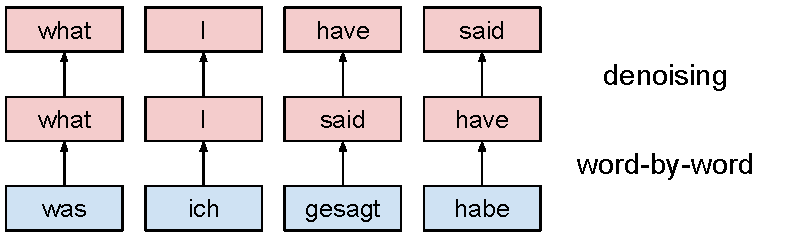
\includegraphics[width=14cm]{denoising}
	\caption{ Reordering noise}
	\centering
\end{figure}
	\textbf{Reordering Noise}\\

	The reordering problem is a common phenomenon in the word-by-word translation since the word order in source language is not the same as in target language. 
	For example, in  the grammar of German, the verb is often placed at the end of the clause. 
	``um etwas zu tun". However in English, it is not the case; the corresponding translation sequence is ``to do something". The verb should always before the noun.
	In our beam search, LM only assists in choosing  more suitable word from the translation candidates, and cannot reorder the word sequence at all.
	
	For a clean sentence from the target monolingual corpora, we corrupt the word sequence by permutation operation. We limit the maximum distance between the original position and its new position.
	
	The design of reordering noise is as followed:
	\begin{enumerate}
		\item For each position ${i}$, sample an integer ${\delta_i}$ from ${[0, d_{per}]}$
		\item Add ${\delta_{i}}$ to index ${i}$ and sort ${i+\delta_{i}}$
		\item Rearrange the words to be in the new positions, to which where indices have been moved
	\end{enumerate}
	
	Reordering actually depends on specific language pair. The reordering noise here just models the most general case.\\
%	However in the experiments we found the performance of the denoising network aimed at such noise is not obvious. The Bleu score before and after the process is close.\\

	
	\textbf{Insertion Noise}\\
	\begin{figure}[ht]
	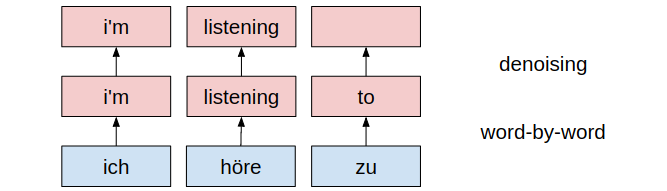
\includegraphics[width=14cm]{insertion}
	\caption{Insertion noise}
	\centering
\end{figure}	

	The word-by-word translation system predict a target word at every source position of the sentence. However,  the vocabularies of different languages are not symmetric. For example, in German, there are more compound words than that in English. So when translating between languages, there are a plenty of cases that a single word will be translated to multiple words and multiple words correspond to a single word conversely. For example: from a German sentence: ``ich höre zu" to ``i'm listening". A very frequent word ``zu" which corresponds to ``to" in English, is dropped from the sentence. The design of insertion noise is as followed:
	\begin{enumerate}	
		\item For each position ${i}$, sample a probability ${p_i \sim \textrm{Uniform}(0,1)}$
		\item If ${p_i} < p_{ins}$, sample a word ${e}$ from the most frequent ${V_{ins}}$ target words and insert it before the position ${i}$
	\end{enumerate}

	We limit the insertion word in a set consisting of the top frequent word in the target language ${V_{ins}}$. Figure 5.2 illustrates the insertion noise.\\
	
	




	\textbf{Deletion Noise}\\
	The deletion noise is just a contrary case of insertion noise.
	Because we are limited to generate only one word per source word, it is also possible that a target word in the reference is not related to any source word.  For example for ``eine der besten" the corresponding translation is ``one of the best". We need to add an extra preposition in the target sentence.  To simulate such situation, we drop some words randomly from a clean target sentence. Figure 5.3 illustrates the deletion noise.\\
	
	\begin{enumerate}
		\item For each position i, sample a probability ${p_i \sim \textrm{Uniform}(0,1)}$
		\item If ${p_i} < p_{del}$, drop the word in the position i
	\end{enumerate}
	
		\begin{figure}[h]
		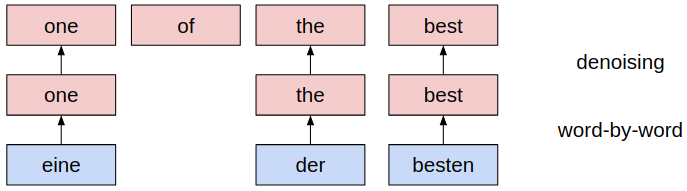
\includegraphics[width=14cm]{deletion}
		\caption{ Deletion noise}
		\centering
	\end{figure}

	
	
	
	
	
	
	
	
	
	
	
	
	
	
	
	
	
	
	
	
	
	
	
	
	
	
	
	
\glsresetall
\chapter{Experiments}
In this chapter, we present experimental results of our proposed methods: corpus-based unsupervised learning algorithm for cross-lingual word embedding and unsupervised MT system integrating LM and DAE. We also empirically analyze the effect of different factors in these methods: corpus size, embedding unit, vocabulary size and artificial noises. Before that, we describe the parameter settings, evaluation methodology, and datasets for our experiments.



\section{Corpus Statistics}
 The training corpora for embedding and LM training are the same, containing 100M sentences
 sampled from News Crawl 2014-2017 monolingual
 corpora. The data was lowercased and filtered
 to have a maximum sentence length 100. The test datasets are for MT evaluation, from WMT 2016   German$\leftrightarrow$English task and WMT 2014 French$\leftrightarrow$English task. We restrict MT vocabulary size to 50k. OOV rates reflect that the vocabulary size we set is reasonable. Each LM perplexity is in the proper range. Detailed statistics are in Table 6.1, 6.2.
\begin{table}[H]
	\centering
	\begin{tabular}{c|c|c|c|c}
		\hline
		\multirow{4}{*}{\textbf{Train}} & \textbf{}              & \textbf{German} & \textbf{English} & \textbf{French} \\ \cline{2-5} 
		& \textbf{Sentences}     & \textbf{100M}   & \textbf{100M}    & \textbf{100M}   \\ \cline{2-5} 
		& \textbf{Running Words} & \textbf{1880M}  & \textbf{2360M}   & \textbf{3017M}  \\ \cline{2-5} 
		& \textbf{Vocabulary}    & \textbf{1254k}  & \textbf{523k}    & \textbf{660k}   \\ \hline
	\end{tabular}
	\caption{Training corpora for embeddings and LM}
\end{table}

\begin{table}[H]
	\centering
	
	\begin{tabular}{c|c|c|c|c|c}
		\hline
		\multirow{7}{*}{\textbf{Test}} & \textbf{}                      & \multicolumn{2}{c|}{\textbf{\texttt{newstest2016}}}    & \multicolumn{2}{c}{\textbf{\texttt{newstest2014}}}    \\ \cline{3-6} 
		& \multicolumn{1}{l|}{\textbf{}} & \textbf{German}       & \textbf{English}      & \textbf{French}       & \textbf{English}      \\ \cline{2-6} 
		& \textbf{Sentences}             & \textbf{2999}         & \textbf{2999}         & \textbf{3003}         & \textbf{3003}         \\ \cline{2-6} 
		& \textbf{Running Words}         & \textbf{62506}        & \textbf{64619}        & \textbf{81165}        & \textbf{71290}        \\ \cline{2-6} 
		& \textbf{Vocabulary Size}       & \textbf{11978}        & \textbf{8645}         & \textbf{10899}        & \textbf{9200}         \\ \cline{2-6} 
		& \textbf{OOV Rates}             & \textbf{4116 (6.6\%)} & \textbf{1643 (2.5\%)} & \textbf{1731 (2.1\%)} & \textbf{1299 (1.8\%)} \\ \cline{2-6} 
		& \textbf{LM perplexity}         & \textbf{211.0}        & \textbf{109.6}        & \textbf{51.2}         & \textbf{84.6}         \\ \hline
		
	\end{tabular}$\texttt{newstest2016}$
	\caption{Evaluation corpora for MT}
\end{table}

\section{Experimental Setup}
We train monoligual word embeddings with a dimensionality of 300 using FastText (\cite{DBLP:journals/corr/BojanowskiGJM16}) for 5 epochs, only for words that have occurs at least 10 times. Our corpus-based approach is also implemented on MUSE framework (\cite{DBLP:journals/corr/abs-1710-04087}). Vocabulary sizes for source and target side are limited to 50k.
$5$-gram LMs are trained separately using KenLM with Kneser–Ney smoothing (\cite{heafield2011kenlm}).\\
LM supported context-aware beam search is performed among top 100 word translation candidates for each position with beam size 10.\\
DAE is implemented in Sockeye (\cite{hieber2017sockeye}), using RNN and Transformer architectures. RNN-based DAE has 2-layer encoder and 2-layer decoder, the hidden layer size is 512. In Transfomer based DAE, encoder and decoder both have 6 layers and hidden layer size is also 512. The multi-head attention mechanism uses 6 heads. DAEs are trained on smaller monolingual corpora containing 20M sentences. \\
We evaluate different cross-lingual embedding learning methods on cross-lingual word retrieval tasks. The datasets are released by \cite{}, which contains dictionaries for 12 language pairs. Each test dictionary contains 1500 unique source words for evaluation.  
\section{Word Translation}
We conduct the cross-lingual word retrieval task on English$\leftrightarrow$German pair. Empirically, we find the best sentence batch size is 1k and the best initial lr is $0.0001$. Numbers in Table 6.3 are the accuracy results, with the same sentence batch size and initial lr. The last three rows are the baseline experiments: adversarial training, adversarial training with refinement, and supervised learning. Dictionary with 5000 unique source words are provided for supervised learning. We run the novel corpus-based approach on a relative small corpus with 50k sentences, sampled from the training corpus. We implement  different lr schedulers. The first one is to start from initial lr, the second one is to inherit the lr after the training on previous batch sentences. We demonstrate the results for German$\rightarrow$ English and English $\rightarrow$ German with the first scheduler, also the performance of  German$\rightarrow$ English with second scheduler.

\begin{table}[H]
	\centering
	\begin{tabular}{llcc}
		\hline
		&                & De-En [\%]& En-De [\%]            \\ \hline
		\multirow{2}{*}{Corpus-based } & lr scheduler 1 & 60.37 & 60.67            \\ \cline{2-4} 
		& lr scheduler 2 & 51.50 & \textbackslash{} \\ \hline
		Corpus-based without LM              & lr scheduler 1 & 54.36 &        \textbackslash{}           \\ \hline
		Adversarial                            &                & 53.50 &       \textbackslash{}   \\ \hline
		Adversarial + Refinement               &                & 64.92 & \textbackslash{}    \\ \hline
		Supervised                             &                & 65.38 & \textbackslash{}  \\ \hline
	\end{tabular}
	\caption{Cross-lingual word retrieval accuracy}
\end{table}
%In general, $1k$ is a option for sentence batch size. The embedding mappings from English to German and from German to English show close results.
%However the second Empirically, we find the best sentence batch size is 1k and initial lrscheduler inheriting last lr works not as well as the first one. We augment training data by training 2 epochs and extending the corpus to 200k sentences. The results are in Table 6.7, the sentence batch size is $1k$ and initial lr are set to $0.0001$, the best settings empirically.\\
%	\end{itemize}
As demonstrated in Table 6.3, the retrieval accuracy of supervised learning is the highest among the results, with iterative refinements the performance of adversarial training proposed by \cite{DBLP:journals/corr/abs-1710-04087} is very close to supervised case. \\
Our corpus-based approach works well, though there is 4\% distance to supervised training. It surpasses the approach using adversarial training only. The first lr scheduler always performs better than the second one, and results for mappings from English to German and from German to English are near, this is what we have expected.  Without LM the corpus-based approach can still learn a mapping, but finally results much worse than that integrating LM.\\

\begin{figure}[h]
	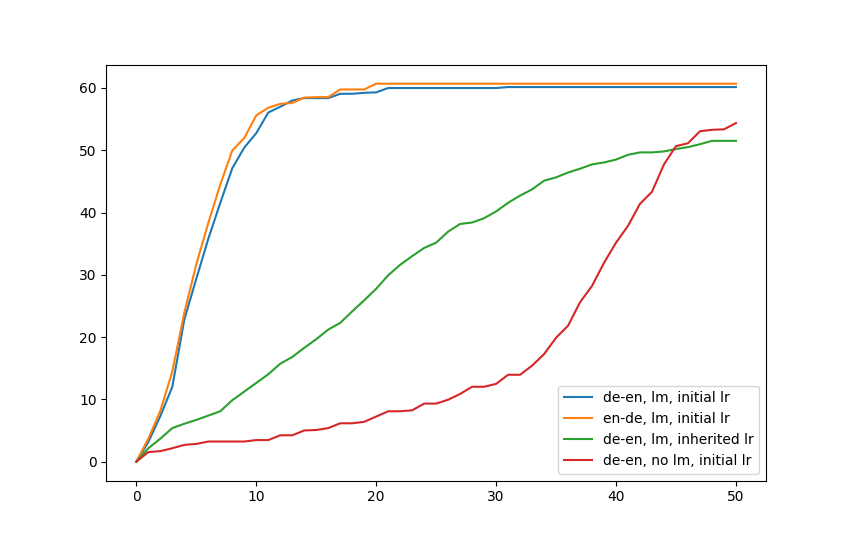
\includegraphics[width=10cm]{corpus}
	\centering
	\caption{Comparison of different experimental settings}
\end{figure}
We plot how retrieval accuracy varies w.r.t the number of training batches in Figure 6.1. The overlapping curves are from corpus-based approach with the first lr sheduler.  Without LM, the green curve increases slowly and converges finally under the normal approach. The curve for the second scheduler increases most slowly at the beginning, and rise obviously after a half of training batches. Since it still keeps increasing, we augment the training data by training for two epochs and extend the corpus size to 200k. The results are shown in Table 6.4.\\

\begin{table}[h]
	\centering
	\begin{tabular}{lc}
		\hline
		Corpus & \textsc{Accuracy} [\%] \\ \hline
		50k    & 51.50         \\ \hline
		50k $\times$2  & 55.51         \\ \hline
		200k   & 57.87         \\ \hline
	\end{tabular}
	\caption{Word retrieval accuracy with different training corpora}
\end{table}
The performance of the second scheduler gets improved when enlarging training data, but is still not so good as the first scheduler.  


\section{Sentence Translation}


\subsection{Overall Results}
\begin{table}[H]
	

	\centering
		\scalebox{0.8}{
		\begin{tabular}{lcccc}
			\toprule
			& De-En & En-De & Fr-En & En-Fr\\
			System   & \textsc{Bleu} [\%] & \textsc{Bleu} [\%] & \textsc{Bleu} [\%] & \textsc{Bleu} [\%]\\
			\midrule
			Word-by-Word   & 11.1 & 6.7 & 10.6 & 7.8\\
			\midrule
			+ LM (5-gram) + tgt w/ high LM score for OOV  & 12.9 & 8.9 & 12.7 & 10.0\\
			+ LM (5-gram) + copy from src for OOV		& 14.5 & 9.9 & 13.6 & 10.9\\
			\midrule
			\hspace{10pt}+ Denoising (RNN)  & 16.2 & 10.6 & 15.8 & 13.3 \\
			\hspace{10pt}+ Denoising (Transformer) & \leavevmode\color{blue}{17.2} & \leavevmode\color{blue}{11.0}& \leavevmode\color{blue}{16.5} & \leavevmode\color{blue}13.9 \\
			\midrule
			\cite{lample2017unsupervised} & 13.3 & 9.6 & 14.3 & 15.1\\
			\cite{artetxe2017unsupervised} & - & - & 15.6 & 15.1\\
			\bottomrule
		\end{tabular}}
	\caption{Translation results on German$\leftrightarrow$English \texttt{newstest2016} and French$\leftrightarrow$English \texttt{newstest2014}}

\end{table}
As demonstrated in Table 6.5, LM improves wordby-word
baselines consistently in all four tasks, giving at least +3\% BLEU. When our denoising
model is applied on top of it, we have additional
gain around +3\% BLEU. Note that our methods
do not involve any decoding steps to generate
pseudo-parallel training data, but still perform
better than unsupervised MT systems that rely on
repetitive back-translations by up to +3.9\% BLEU.
%above, our unsupervised MT surpass the start-of-the-art unsupervised NMT in almost all cases except English$\rightarrow$French translation. Each sub-model lift the performance respectively. Copy OOV word from source sentences works better than those predicted by language model, because OOV words are usually specific name entities and LM prefers common words rather than rare words. Denoising autoencoder based on Transformer structure outputs better translation than the traditional RNN structure. 


	\begin{table}[!h]
	\centering
	
	\begin{tabular}{ccc}
		\hline
		&\textsc{Accuracy} [\%]& \textsc{Bleu} [\%] \\ \hline
		5M & 44.9  & 9.7  \\ \hline
		10M & 51.6 & 10.1 \\ \hline
		50M & 59.4 & 10.8 \\ \hline
		100M &\leavevmode\color{blue}61.2 & \leavevmode\color{blue}11.2 \\ \hline
	\end{tabular}
\caption {Word-by-word translation from German to English}
\end{table}
As in Table 6.9, larger corpus improves the word translation accuracy as well as the word-by-word translation. 

\subsection{BPE vs Word}
Byte pair encoding (BPE)(\cite{sennrich2015neural}) is a simple data compression technique for word segmentation. It allows for the representation of an open vocabulary through a fixed-size vocabulary of variable-character sequences, making it very suitable word segmentation strategy for neural network models. It helps to reduce the vocabulary size and they eliminate the presence of unknown words in the output translation. We use BPE to represent the mapping between languages and compare with word-level cross-lingual embeddings. In BPE algorithm, the vocabulary is updated using an iterative greedy algorithm. Merges in Table 6.7 denotes the pre-defined number of merge operations. 
	\begin{table}[h]

	\centering
	\scalebox{1}{
		\begin{tabular}{lcc}
			\toprule
			\multicolumn{2}{c}{\textbf{Vocabulary}} & \textsc{Bleu} [\%] \\
			\midrule
			& Merges \\
			\cmidrule{2-2}
			\multirow{3}{*}{BPE} & 
			20k & 10.4 \\
			& 50k & 12.5 \\
			& 100k & \leavevmode\color{blue}13.0 \\
			\midrule
			& Cross-lingual training \\
			\cmidrule{2-2}
			\multirow{4}{*}{Word} & 20k & 14.4\\
			& 50k & 14.4\\
			& 100k & \leavevmode\color{blue}14.5\\
			& 200k & 14.4\\
			\bottomrule
		\end{tabular}
	
	}\\
	\caption{Translation results with different vocabularies.}
\end{table}


%As in Table 6.10, the BPE performs worse than word in this unsupervised learning scenario. It might be difficult to learn the translation relationship between subword units. Also for sentence translation, larger vocabulary size does not improve the performance. In order to balance the efficiency and accuracy we limit the vocabulary size to 50k. To improve the results, LM are exploited here.
We examine how the translation performance varies with different vocabularies of cross-lingual word embedding in Table 6.7. The first three show that BPE embeddings performs worse than word embeddings, especially with smaller vocabulary size. For small BPE tokens (1-3 characters),
the context they meet during the embedding
training is much more various than a complete word, and a direct translation of such small
token to a BPE token of another language would be very ambiguous. For word level embeddings, we compared different vocabulary sizes used for training the
cross-lingual mapping. Surprisingly, cross-lingual word embedding learned only on top 20k words is comparable to that of 200k words in the translation quality. This means that word-by-word translation with crosslingual embedding depends highly on the frequent word mappings, and learning the mapping between rare words does not have a positive effect. 

\subsection{Artificial Noise}

	\begin{table}[H]

	\centering
			\scalebox{1}{
	\begin{tabular}{cccrc}
		\toprule
		$d_\text{per}$ & $p_\text{del}$ & $p_\text{ins}$ & $V_\text{ins}$ & \textsc{Bleu} [\%] \\
		\midrule
		2 & & & & 14.7\\
		3 & & & & \leavevmode\color{blue}{14.9}\\
		5 & & & & 14.9\\
		\midrule
		\multirow{2}{*}{3} & 0.1 & &  & \leavevmode\color{blue}{15.7} \\
		& 0.3 & & & 15.1 \\
		\midrule
		\multirow{4}{*}{3} & \multirow{4}{*}{0.1} & \multirow{4}{*}{0.1} & 10 & 16.8 \\
		& & & 50 & \leavevmode\color{blue}{17.2} \\
		& & & 500 & 16.8 \\
		& & & 5000 & 16.5\\
		\bottomrule
	\end{tabular}
}

	\label{tab:denoising}
		\caption{ Translation results with different values of denoising
			parameters.}
\end{table}
To examine the effect of each noise type in denoising
autoencoder, we tuned each parameter of the noise and combined them incrementally as in Table 6.8.  Firstly, for permutations, a significant improvement is achieved from $d_{per}$ = 3, since a local
reordering usually involves a sequence of 3 to 4
words. With $d_{per} \le 5$ , it shuffles too many consecutive
words together, yielding no further improvement.
This noise cannot handle long-range reordering, which is usually a swap of words that are far from each other, keeping the words in the
middle as they are. \\
Secondly, we applied the deletion noise with
different values of $p_{del}$. 0.1 gives +0.8\% BLEU, but we immediately see a degradation with a larger value; it is hard to observe more than one one-tomany
translations in each German→English sentence pair.
Finally, we tested several sizes of $V_{ins}$ for the
insertion noise, fixing $p_{ins}$ = 0.1. Increasing $V_{ins}$
is generally not beneficial, since it provides too
much variations in the inserted word, which might
not be related to its neighboring words. Overall,
we observe the best result (+1.5\% BLEU) with
$V_{ins} = 50$.



\subsection{Phrase Embedding}

\begin{table}[h]
	\centering
	\begin{tabular}{ccccc  c}
		\hline
		\multicolumn{3}{c}{\multirow{2}{*}{\textbf{Vocabulary}}}                  & No LM & With LM & Denoising \\
		\multicolumn{3}{c}{}                                         &  \textsc{Bleu} [\%]  &  \textsc{Bleu} [\%] & \textsc{Bleu} [\%]   \\ \hline
		Word            & \multicolumn{2}{l}{}              & 11.2 & 14.5  &\leavevmode\color{blue}{ 17.2} \\
		\hline
		\multirow{3}{*}{\cite{mikolov2013distributed} } & \multirow{3}{*}{threshold} & 100  & 11.1 & 13.7  & 15.6 \\ \cline{3-6} 
		&                            & 500  & 11.0 & 13.7  & 16.2 \\ \cline{3-6} 
		&                            & 2000 & 10.7 & 14.0  &16.5 \\ \hline
		Top frequent              & \multicolumn{1}{l}{\text{count}}  & 50k  & \leavevmode\color{blue}12.0 & \leavevmode\color{blue}15.7  & 16.8 \\ \hline
	\end{tabular}
	\caption{Performance of phrase embedding in MT.}
\end{table}
%With word2vec tool (\cite{mikolov2013distributed}) we detect phrases in the training corpus. We set threshold value to 100, 500, 2000 to make the number of phrases differs. Fewer phrases will be detected as we lift the threshold value. As to our method, we extract only bigrams that in the top 50k frequent bigrams in the training corpus. We learn phrase embedding in an unsupervised manner as normal word embedding. \\
%As demonstrates in Table
We examine how phrase embedding performs in MT. Phrase embedding using detection technique proposed by \cite{mikolov2013distributed} works better if we lift up the threshold value. The performance of MT gets harmed when too many phrases. And the results is even worse than word embedding.  While with our phrase detection method, BLEU of MT results is higher when using word-by-word translation and integrating LM. The final results are denoising step is not as good as word embedding. 
%?????? not sure if I need to add this corresponding part in unsupervised cross-lingual embedding


%\subsection{Vocabulary Cutoff in Translation}
%\begin{table}[h]
%	\parbox{.5\linewidth}{
%		\centering
%		\caption{Word embedding vocabulary cut-off}
%		\begin{tabular}{c c c c } 
%			\hline
%			\textsc{Bleu} [\%]	& 20k & 50k & 100k \\
%			\hline
%			50k &	11.1  & \leavevmode\color{blue}11.3 & 11.2  \\ 
%			\hline
%			100k&	11.2  & 11.2 & 11.1 \\ 			
%			\hline
%			150k&	10.9 & 10.9 & - \\
%			\hline
%		\end{tabular}
%		
%	}
%	\hfill
%	\parbox{.5\linewidth}{
%		\centering
%		\caption{Phrase embedding vocabulary cut-off}
%		\begin{tabular}{c c c c } 
%			\hline
%			\textsc{Bleu} [\%]	& 50k & 100k & 150k \\
%			\hline
%			50k &	11.3  & - & -  \\ 
%			\hline
%			100k&	11.9  & 11.9 & - \\ 			
%			\hline
%			150k&	\leavevmode\color{blue}12.0 & 11.9 & 11.9 \\
%			\hline
%			200k & 12.0 & - & - \\
%			\hline
%		\end{tabular}
%		
%	}
%\end{table}


\glsresetall
\chapter{Conclusion}


For unsupervised machine translation system, the context-aware beam search language model help at the lexicon choice step.\\
The denoising networks which aimed at the insertion/deletion/reordering noise in the word-by-word translation sentence works well for fertility and localized reordering problem. 
Even though BPE is known to be an effective way to overcome the rare word problem in standard NMT, BPE embedding performs worse than word embedding in our case especially when vocabulary is small.\\
Word-by-word translation based on cross-lingual word embedding depends highly on the frequent word mappings. We found that phrase embedding only helps in word-by-word translation with context-aware beam search, it works not as good as that under the processing of denoising autoencoder.

\appendix
\chapter{Appendix}



\backmatter          % Nachspann einleiten (wie frontmatter)
\listoffigures
\listoftables

% \nocite{*}



\bibliographystyle{plainnat}
\bibliography{references}

\end{document}
